\documentclass[
   technote
]{phildoc}
\def\Restriction   {2}                      % Enter 0= Unclassified, 1= Philips restricted, 2= Company Confidential
\def\Noteno        {xxxx}                   % Report number
\def\Noteyr        {2016}                   % Report year
\def\Miss          {09}                     % Month issued
\def\Yiss          {}                   % Year issued
\def\Maintitle     {A Machine Learning Algorithm for the Early Detection of Acute Kidney Injury (AKI) in the Pediatric Intensive Care Unit (PICU)}
\def\Subtitle      {}
\def\Authorname    {Byung Gu Cho, Cristhian Potes}
\def\Authormail    {byung.gu.cho@philips.com}
\def\Audept        {Philips Research North America, Acute Care Solutions}
\def\Mcfunt        {}            % Company Confidential until month
\def\Ycfunt        {}          % Company Confidential until year
\def\Reviewernames {}
\def\Additionalnos {}
\def\Subcategory   {}
\def\Project       {}
\def\Customer      {Patient Care Monitoring Solutions}
\def\Keywords      {acute kidney injury}
\def\Conclusion    {}
\def\Abstract{

}

\usepackage[utf8]{inputenc}
\usepackage{multirow}
\newcommand{\ie}{i.e.,}
\newcommand{\eg}{e.g.,}
\newcommand{\hii}{HII}
\newcommand{\pedAKI}{PED-AKI}
\newcommand{\apriori}{\textit{a priori}}
\newcommand{\keyw}[1]{{\bf #1}}
\newcommand{\rsquared}{$r^{2}$}
\newcommand{\fig}{Fig.}
\newcommand{\tab}{Table}
\newcommand{\eq}{Eq.}
\newcommand{\matlab}{Matlab\texttrademark}

\chapterstyle{section}  % chapters typeset less pronounced
\tightlists             % tighter lists
\unitlength=1.5em       % for the picture environment
\usepackage{hyperref}
\usepackage{memhfixc}
\usepackage{amsfonts}
\usepackage{amssymb}
\usepackage{amsmath}
%\usepackage{pdflscape}
%\usepackage{latexsym}
%\usepackage{color}
%\usepackage{algorithm}
%\usepackage{algpseudocode}
%\usepackage[tight]{subfigure}
%\usepackage{verbatim}
%\usepackage{multicol}
\usepackage{bm}
%\usepackage{amssymb}
\usepackage{listings}
\usepackage{color} %red, green, blue, yellow, cyan, magenta, black, white
\usepackage{graphics}
\usepackage{graphicx}
\usepackage{threeparttable}

%\usepackage[table]{xcolor}
%\usepackage{epsfig}

\definecolor{mygreen}{RGB}{28,172,0} % color values Red, Green, Blue
\definecolor{mylilas}{RGB}{170,55,241}

\definecolor{darkgreen}{rgb}{0,0.5,0}
\newcommand{\mx}[1]{{\color{green}{MX: #1}}}
\newcommand{\bc}[1]{{\color{cyan}{BC: #1}}}
\newcommand{\ly}[1]{{\color{red}{LY: #1}}}
\newcommand{\rf}[1]{{\color{blue}{RF: #1}}}
% To insert a comment use it as \mx{insert comment}

\def\ck{+}%\checkmark}
\MakeShortVerb{|}

\begin{document}

\Tnotefrontmatter
\Large

\chapter{Introduction}
\label{Introdution}
Acute Kidney Injury (AKI) is known as an independent indicator that is closely associated with mortality \cite{sanchez2015association}. Therefore, early prediction of AKI is important for clinicians to apply appropriate treatments before the patient deteriorates. The main biomarker of AKI, serum creatinine (SCr), is unfortunately a late marker of injury, which delays early diagnosis and treatment. Recently, there has been an attempt for early detection of AKI using Electronic Health Records (EHR) data from PICU patients \cite{sanchez2016development}.
\begin{enumerate}
\item CAUSE OF AKI
\item COMPENSATORY MECHANISM
\item TREATMENTS: What are the treatments? When does the intervention happen? If we can predict in advance, can there be a differnce? If so, what is the  minimum timewindow needed in order to make a difference by providing prediction?
\item CHALLENGES: There are several AKI staging criterion that are used among clinicians. Which one should we use for the algorithm? Are they totally different from each other? How is baseline creatinine defined? Is there a golden standard for this? How does the clinician
\item AIM: Aim of this project is to create an AKI prediction algorithm for pediatric ICU patients, sot that clinicians can intervene before patient detorioration. 
\end{enumerate}
\section{Definitions}
\begin{itemize}
\item A \textbf{clinical feature} is defined as a clinical event that has a value, unit of measurement, and time when it was measured and/or recorded. Examples of clinical features are heart rate, systolic blood pressure, glucose, etc. 
\item A \textbf{clinical encounter} is defined as any physical or virtual contact between a patient and healthcare practitioner, during which an assesment or clinical activity is performed. Each clnical encounter consists of vital signs, laboratory values, and demographic information about the patient. Note that a single patient can have multiple clinical encounters.
\item An \textbf{example} is a subset of clinical encounter that is refined and structured for training and testing the learning algorithm. An example is composed of features (\ie{} predictors) and a binary label that indicates whether the encounter experienced AKI or not.
\item \textbf{Acute Kidney Injury (AKI)}, formerly called Acute Renal Failure (ARF), is commonly defined as an abrupt decline in renal function, clinically manifesting as a reversible acute increase in nitrogen waste products—measured by Blood Urea Nitrogen (BUN) and serum creatinine levels—over the course of hours to weeks. The vague nature of this definition has historically made it difficult to compare between scholarly works and to generalize findings on epidemiologic studies of AKI to patient populations. Several classification systems, such as KDIGO, AKIN, and RIFLE, have been developed to streamline research and clinical practice with respect to AKI. 
\item A \textbf{clinical intervention} is defined as any treatment to manage AKI. This includes correction of fluid overload with furosemide, correction of severe acidosis with bicarbonate administration, which can be important as a bridge to dialysis, correction of hyperkalemia, and correction of hematologic abnormalities (eg, anemia, uremic platelet dysfunction) with measures such as transfusions and administration of desmopressin or estrogens.
\end{itemize}

\section{Team}


\section{Intended Audience}
This document is intended for scientists and engineers at Philips who would like to know the details, performance, and architecture of the algorithm. General understanding of machine learning techniques and physiology is helpful for understanding this document. 

% This data-driven prediction model can be implemented in the workflow of clinicians in a form of advanced Clinical Decision Support (CDS) systems.


\chapter{Materials and Methods}
\label{methods}
\section{Data Compilation}
\label{sec:data_compilation}
We used dataset from patients admitted to the Pediatric Intensive Care Unit (PICU) in three hospitals for training and validating the pediatric AKI prediction model. Data sets were from the PICU at Children's Hospital at Los Angeles (CHLA) from 2003 to 2011, St.Mary's Hospital at London, UK, and Banner hostpital at \textbf{??}. 

% EHR data of patients between 1 month to 21 years old that stayed at the ICU for at least 24 hours between May 2003 and March 2015 \cite{sanchez2016development}. Data set is a mixture of patients with medical, surgical trauma, solid organ and stem cell transplantation, but not postoperative cardiac patients. Patients were excluded if they had AKI on admission, had documented chronic kidney disease, were perioperative for a kidney transplant, or hand no SCr levels measured. The first 12 hour EHR data was used for the prediction model.

\subsection{Data from CHLA}
The dataset from CHLA was obtained retrospectively from an electronic flow sheet (Philips Care-Vue, Waltham, MA) and a hospital-owned database (Microsoft Access, Redmond,WA)). This dataset includes records from patients (13,323 patients and 16,842 encounters) admitted to the PICU at Children’s Hospital Los Angeles (CHLA) from 2003 to 2011. A patient could have more than one encounter. We refined the data set to include only the patients whose age at admission was between 1 month and 21 years old and had a recorded creatinine level. Only the encounters with length of stay at PICU longer than 24 hours were chosen. For patients with more than a single encounter, the encounter with the longest length of stay at PICU was chosen such that each patient has a single encounter. 

AKI stage, either 1,2, or 3, was annotated to each creatinine level measurement according to the Kidney Disease Improving Global Outcomes (KDIGO) AKI staging criteria \cite{kdigo2012guideline} as shown in \tab{} \ref{tab:AKI_def}. AKI stage 0 was annotated if the creatinine level doesn't fall into any of the KDIGO AKI stages. Baseline creatinine was determined by the upper limit of normal creatinine level for age and gender group \cite{schwartz1976plasma, bellomo2004acute, schneider2010serum} as shown in \tab{} \ref{tab:bs_scr}. Rate of change of creatinine within the past 48 hours was determined by calculating the slope (mg/dL/hour) of a line least square fitted to the creatinine measurements within the past 48 hours from each creatinine measurement time, and multiplied by 48 hours. The past 48 hours time window for each creatinine measurment was defined as $\left[\text{creatinine measurement time - 48 hours}, \text{creatinine measurement time} \right]$, where the square brackets $\left[ \right.$ and $\left. \right]$ indicate inclusion of the boundary. Initiation of renal replacement therapy and glomerular filtration rate were not used for AKI staging in the current implementation due to lack of information. For example, for an encounter that has $m$ creatinine measurements over the stay at PICU has $m$ AKI stages annotated to each creatinine measurement according to the KDIGO AKI staging criteria. 

\begin{table}[!htbp]
\centering
\caption{KDIGO AKI Staging Criteria}
\label{tab:AKI_def}
\begin{tabular}{|c | p{7cm}|}
\hline
Acute Kidney Injury Stage & Kidney Disease Improving Global Outcomes (KDIGO) Criteria \\ \hline \hline
\multirow{2}{*}{1}
& $\geq$1.5 and $<$1.9 times baselines SCr* OR \\
& $\geq$0.3 mg/dL increase in SCr within 48 hours \\ \hline
2 & $\geq$2.0 and $<$2.9 times baseline SCr \\ \hline
\multirow{4}{*}{3}
& $\geq$3.0 times baseline SCr OR \\
& Increase in SCr to $\geq$4.0 mg/dL OR \\
& Initiation of renal replacement therapy OR \\
& In patients $<$18 yr, decrease in estimated glomerular filtration rate $<$35 mL/min per 1.73 m$^2$. \\ \hline

\multicolumn{2}{p{11.5cm}}{\vspace{0.1em} * Baseline creatinine is defined as $\max{}$(the most recent documented SCr within 6 months of the ICU admission, the low normal for age and gender). If a prior SCr was unavailable, the upper limit of normal for age and gender was used.}
\end{tabular}
\end{table}


\begin{table}[! htbp] \centering \caption{Normal Creatinine Range} \label{tab:bs_scr}
\begin{threeparttable}
\begin{tabular}{| l | l | l |}
\hline
Age & Range & Units \\ \hline \hline
Premature & 0.3-1.0 & mg/dL \\
Neonates & 0.2-0.9 & mg/dL \\
$\left[\right.\text{1 month, 1 year} \left. \right)$ & 0.2-0.4 & mg/dL \\
$\left[\right. \text{1 year, 3 years} \left. \right)$ & 0.2-0.5 & mg/dL \\
$\left[\right. \text{3 years, 5 years} \left. \right)$ & 0.3-0.7 & mg/dL \\
$\left[\right. \text{5 years, 7 years} \left. \right)$ & 0.3-0.7 & mg/dL \\
$\left[\right. \text{7 years, 9 years} \left. \right)$ & 0.2-0.6 & mg/dL \\
$\left[\right. \text{9 years, 11 years} \left. \right)$ & 0.3-0.7 & mg/dL \\
$\left[\right. \text{11 years, 13 years} \left. \right)$ & 0.3-0.9 & mg/dL \\
$\left[\right. \text{13 years, 16 years} \left. \right)$ & 0.4-0.9 & mg/dL \\
$\geq$16 years, Males & 0.6-1.2 & mg/dL \\
$\geq$16 years, Females & 0.5-1.0 & mg/dL \\ \hline
\end{tabular}
\begin{tablenotes}
\item[*] Age is defined as the time since born. Square bracket, [ and ],  indicates inclusion of the boundary value and parenthesis, ( and ), indicates exclusion of the boundary value. Note that there are gender specific ranges only for age $\geq$ 16.
\end{tablenotes}
\end{threeparttable}
\end{table}

Once AKI stage was annotated for each creatinine measurement, each encounter was labeled as either AKI (\ie{} experimental group) or stable (\ie{} control group). An encounter was labeled as AKI if there is at least one AKI stage$>0$ for the encounter. Otherwise, if the encounter had no AKI stage$>0$, the encounter was labeled as stable. AKI onset of an encounter was defined as the first time stamp at which AKI stage$>0$. Then, patients that were stable at least for the first 12 hours from admission were exclusively considered in order to investigate patients who have developed AKI after their admission to PICU. In other words, if the time difference between AKI onset and time of admission was less than 12 hours, the encounter was filtered out.

Summary of patient demographics is shown in \tab \ref{tab:demographics_chla}. The final dataset included $8,104$ patients (encounters), where $7,341$ were stable and $763$ had AKI during their PICU stay (AKI group prevalence is 9.4$\%$). Among the $8,104$ patients,  $4,426$ were males, $3,678$ were females. The average length of stay in the PICU was $29.96$ days for the AKI group, and $7.48$ days for the stable group. Number of patients on ventilator was determined by counting the patients with Mean Airway Pressure (MAP).
% Age distribution for AKI and stable patients is shown in \fig{} \ref{fig:histogram_age_chla}.

\begin{table}[!htbp] \centering \caption{Demographics of AKI group and stable group from CHLA} \label{tab:demographics_chla}
\begin{tabular}{| l | l | l |}
\hline
\textbf{Group} & \textbf{AKI} & \textbf{Control}\\
\hline \hline
Total patients (January 2003 to January 2011) & 763 & 7,341 \\
\hline
Total encounters	&	763	& 	7,341  \\
\hline
Prevlanece of AKI patients
& 9.4 \% & 90.6 \% \\
& Stage 1: 519 (6.4 \%) & \\
& $\;\;$ by SCr value: 52 (0.6 \%) & \\
& $\;\;$ by SCr rate: 467 (5.8 \%) & \\
& Stage $>$1: 244 (3 \%) & \\
\hline
Male (\%) 			& 	414/763 (54.3 \%)		&	4012/7341 (54.7 \%)	\\
\hline
Female (\%)		&	349/763 (45.7 \%)		&	3329/7341 (45.3 \%)	 \\
\hline
Age (years)		&	6.49 	&	6.39  \\
\hline
Length of PICU stay (days)	& 29.96 &	7.48 \\
\hline
Patients on ventilator (\%) & 651/763 (85.3 \%) & 3852/7341 (52.5 \%) \\
\hline
Mortality (\%) & 150/763 (19.7 \%) & 172/7341 (2.3 \%) \\
\hline
\end{tabular}
\end{table}

%\begin{figure}[!htbp]
%\centering
%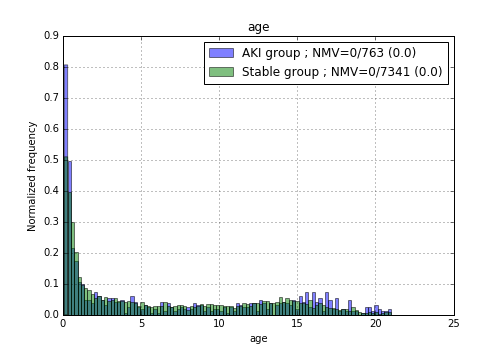
\includegraphics[width=6in]{../figures/histogram_age_chla.png}
%\caption{Age distribution for the AKI and stable groups (y-axis corresponds to the number of encounters divided by the total number of encounters within each group, and x-axis corresponds to age in years). Pruple bars correspond to AKI encounters and green bars correspond to stable encounters.} 
%\label{fig:histogram_age_chla}      
%\end{figure}

Each encounter was refined and structured to from an example for training and testing the AKI prediction algorithm. An example comprised 111 features (\ie{} predictors) and a binary label that indicates whether the example falls into the AKI group or stable group. 111 features include vital signs, laboratory values, and demographic information of the patient. Value of each feature was extracted within an observation window which precedes the AKI onset by the prediction window. Observation window was defined as the time window during which the feature values were extracted. Prediction window was defined as the time difference between the AKI onset and the end of observation window. Illustrative example of AKI onset time, 6 hour observation window, and 12 hour prediction window is depicted in \fig{}\ref{fig:data_extraction}. Current implementation used observation window of 6 or 12 hours and prediction window ranging from 6 to 18 hours. Missing value (\ie{} Not a Number (NaN)) was assigned to a feature in an example if no measurements were found within the observation window for that feature in the example. A similar procedure was applied to extract features from the stable group, but assigning the reference time. For the stable group, there was no AKI onset, therefore reference time was assigned randomly for each encounter. Once the reference time for each encounter was assigned, identical procedure was applied to form examples. Examples were then complied to form a design matrix $X$ and label vector $y$.  $X$ is a $p$ by $N$ matrix, where $p$ is the number of features (\ie{} $p=111$) and $N$ is the total number of examples. y is a column vector of length $N$, where $y^{(i)} \in \lbrace{ 0, 1\rbrace}$ ($y^{(i)}=0$ indicates the example was stable, whereas $y^{(i)}=1$ indicates the example had AKI).

Shock Index (SI), Oxygenation Index (OI), and Oxygen Saturation Index (OSI) were the composite variables that were derived from a combination of multiple variables. For instance, SI is the Heart Rate (HR) per unit non Systolic Blood Pressure (nSBP), \ie{} $\displaystyle\text{SI} = \frac{\text{HR}}{\text{nSBP}}$, where the unit of measurement was bpm/mmHg. When the timestamps of HR and nSBP didn't coincide, SI values were calculated from the HR and nSBP values that were closest to each other within an hour. Otherwise, a NaN was assigned. OI is a measure of required partial pressure of oxygen in the airway per unit partial pressure of oxygen in arterial blood, \ie{} $\displaystyle \text{OI} = \frac{\text{FiO}_2 \times\text{MAP}}{\text{PaO}_2}\times 100$ (\%). Similarly, OSI is a measure of required partial pressure of oxygen in the airway per unit oxygen saturation level, \ie{} $\displaystyle \text{OSI} = \frac{\text{FiO}_2 \times\text{MAP}}{\text{SpO}_2}\times 100 \left(\text{cmH}_2\text{O}\right)$. Similar to how SI was calculated, OI and OSI values were calculated using the closest MAP, $\text{FiO}_2$, and $\text{PaO}_2$ or $\text{SpO}_2$ values within an hour when the timestamps did not coincide. Otherwise, NaN was assigned.



\begin{figure}[htbp!]
	\centering
	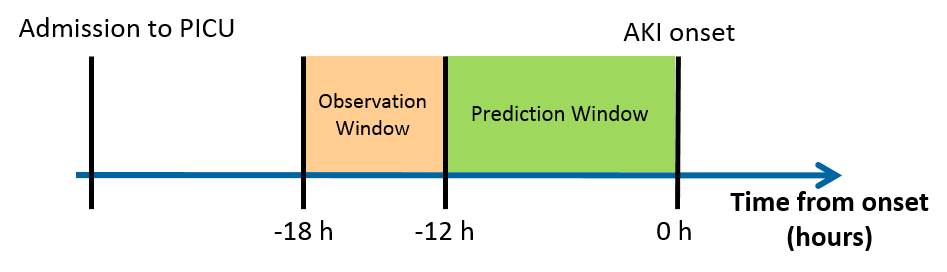
\includegraphics[width=6in]{./figures/data_extraction.png}
	\caption{Data Extraction} 
	\label{fig:data_extraction}      
\end{figure} 

Known risk factors of kidney injury that were available in Electronic Health Records (EHR) were chosen as pathophysiological variables \cite{sanchez2016development}. Mean, maximum, minimum, and last values within the observation window for each pathophysiological variable (except age) were chosen as features. (See \tab \ref{tab:features} for the full list of 111 features).

\begin{table}[!htbp] \centering \caption{List of features used for AKI prediction, along with their units of measurement, percentage of patients with that feature recorded, and representative statistics over the observation window that were included as a feature.}
\label{tab:features}
\begin{tabular}{| l | l | l | l |  }
\hline
\multicolumn{4}{|c|}{\textbf{Arterial Blood Gas}} \\
\hline
Arterial pH					&			&	31	&	Mean, Maximum, Minimum, Median, Last\\

\hline
\multicolumn{4}{|c|}{\textbf{Ventilator Parameters}} \\
\hline
PF ratio					&						&	32	&	Mean, Maximum, Minimum, Median, Last\\
Oxygenation Index (OI)		&						&	9	&	Mean, Maximum, Minimum, Median, Last\\
Oxygen Saturation Index (OSI)	&	$\text{cmH}_2\text{O}$	&	25	&	Mean, Maximum, Minimum, Median, Last\\

\hline
\multicolumn{4}{|c|}{\textbf{Basic Metabolic Panel}} \\
\hline
Blood Urea Nitrogen (BUN)		&	mg/dL	&	23	&	Mean, Maximum, Minimum, Median, Last\\
Creatinine					&	mg/dL	&	23	&	Mean, Maximum, Minimum, Median, Last\\
Potassium					&	meq/L	&	40	&	Mean, Maximum, Minimum, Median, Last\\
Glucose					&	mg/dL	&	25	&	Mean, Maximum, Minimum, Median, Last\\
Calcium					&	mg/dL	&	23	&	Mean, Maximum, Minimum, Median, Last\\

\hline
\multicolumn{4}{|c|}{\textbf{Complete Blood Count}} \\
\hline
WBC - Leukocytes			&	K/$\mu$L	&	23	&	Mean, Maximum, Minimum, Median, Last\\
Platelets					&	K/$\mu$L	&	24	&	Mean, Maximum, Minimum, Median, Last\\
Hemoglobin				&	g/dL		&	25	&	Mean, Maximum, Minimum, Median, Last\\

\hline
\multicolumn{4}{|c|}{\textbf{Noninvasive Vitals / Demographics}} \\
\hline
Noninvasive Systolic Blood Pressure (nSBP)	&	mmHg		&	77	&	Mean, Maximum, Minimum, Median, Last\\
Noninvasive Diastolic Blood Pressure (nDBP)	&	mmHg		&	77	&	Mean, Maximum, Minimum, Median, Last\\
Heart Rate (HR)						&	bpm			&	93	&	Mean, Maximum, Minimum, Median, Last\\
Noninvasive Shock Index (SI)			&	bpm/mmHg	&	77	&	Mean, Maximum, Minimum, Median, Last\\
$\text{SpO}_2$						&	\%			&	61	&	Mean, Maximum, Minimum, Median, Last\\
Temperature (T)					&	$^\circ$C		&	93	&	Mean, Maximum, Minimum, Median, Last\\
Age								&				&	100	&	\\



\hline
\multicolumn{4}{|c|}{\textbf{Additional Tests}} \\
\hline
Lactic Acid					&	mg/dL	&	1	&	Mean, Maximum, Minimum, Median, Last\\
Urine Output				&	cc/kg/hr	&	74	&	Mean, Maximum, Minimum, Median, Last\\

\hline
\multicolumn{4}{|c|}{\textbf{Comprehensive Metabolic Panel}} \\
\hline
Albumin					&	g/dL		&	5	&	Mean, Maximum, Minimum, Median, Last\\
Bilirubin					&	mg/dL	&	4	&	Mean, Maximum, Minimum, Median, Last\\

\hline

\end{tabular}
\end{table}

\subsection{Data from St.Mary's Hospital}
This dataset includes records from patients (2,094 patients and 2,435 encounters) admitted to the PICU at St.Mary's hospital. Data extraction and refinement procedure for CHLA dataset was identically applied to the St.Mary's data set. Only patients whose age at admission was between 1 month and 21 years and had recorded creatinine level were considered. Only patients who stayed at the PICU more than 24 hours and stable for at least for the first 12 hours from PICU admission were considered. For patients who had multiple encounters, only the encounter that had the longest length of stay at PICU was picked. 

Summary of patient demographics is shown in \tab \ref{tab:demographics_stm}. The final dataset included $1,388$ patients (encounters), where $1,225$ were stable and $163$ had AKI during their PICU stay (AKI group prevalence is 11.7$\%$). Among the $1,388$ patients,  $768$ were males, $620$ were females. The average length of stay in the PICU was $20.38$ days for the AKI group, and $6.06$ days for the stable group. 
%Age distribution for AKI and stable patients is shown in \fig{} \ref{fig:histogram_age_stm}.

\begin{table}[!htbp] \centering \caption{Demographics of AKI group and stable group from St.Mary's} \label{tab:demographics_stm}
\begin{tabular}{| l | l | l |}
\hline
\textbf{Group} & \textbf{AKI} & \textbf{Control}\\
\hline \hline
Total patients & 163 & 1,225 \\
\hline
Total encounters	&	163	& 	1,225  \\
\hline
Prevlanece of AKI patients
& 11.7 \% & 88.3 \% \\
& Stage 1: 123 (8.9 \%) & \\
& $\;\;$ by SCr value: 78 (5.6 \%) & \\
& $\;\;$ by SCr rate: 45 (3.3 \%) & \\
& Stage $>$1: 40 (2.9 \%) & \\
\hline
Male (\%) 			& 	85/163 (52.1 \%)		&	683/1225 (55.8 \%)	\\
\hline
Female (\%)		&	78/163 (47.9 \%)		&	542/1225 (44.2 \%)	 \\
\hline
Age (years)		&	4.71 	&	4.00  \\
\hline
Length of PICU stay (days)	& 20.38 &	6.06 \\
\hline
Patients on ventilator	& 158/163 (96.9 \%) &	1037/1225 (84.7 \%) \\
\hline
Mortality & 32/163 (19.6 \%) & 36/1225 (2.9 \%) \\
\hline
\end{tabular}
\end{table}

Some features were present in in CHLA data set but missing in St.Mary's data set. Arterial pH, Calcium, BUN, and bilirubin were missing in St.Mary's data set. PF ratio was present in both data sets, however, the conversion factor between the two data sets was not consistent with the conversion factors among commonly used unit of measurements of PF ratio. Below shows the 18 features that were present in both CHLA and St.Mary's data sets.

\subsection{Data from Banner Hospital}
This dataset includes records from patients admitted to the PICU at Banner hospital. Data extraction and refinement procedure for CHLA dataset was identically applied. Only patients whose age at admission was between 1 month and 21 years and had recorded creatinine level were considered. Only patients who stayed at the PICU more than 24 hours and stable for at least for the first 12 hours from PICU admission were considered. For patients who had multiple encounters, only the encounter that had the longest length of stay at PICU was picked. 

Summary of patient demographics is shown in \tab \ref{tab:demographics_banner}. The final dataset included $1,655$ patients (encounters), where $1,593$ were stable and $62$ developed AKI during their PICU stay (AKI group prevalence is 3.8$\%$). Among the $1,655$ patients,  $908$ were males, $747$ were females. The average length of stay in the PICU was $21.66$ days for the AKI group, and $5.37$ days for the stable group. MAP values were missing for most of the patients. There were only 4 patients that had recorded MAP values (2 from AKI group and 2 from Control group). OSI and OI were missing because these features were derived from MAP.

\begin{table}[!htbp] \centering \caption{Demographics of AKI group and stable group from Banner hospital} \label{tab:demographics_banner}
\begin{tabular}{| l | l | l |}
\hline
\textbf{Group} & \textbf{AKI} & \textbf{Control}\\
\hline \hline
Total patients & 62 & 1,593 \\
\hline
Total encounters	&	62	& 	1,593  \\
\hline
Prevlanece of AKI patients
& 3.8 \% & 96.2 \% \\
& Stage 1: 56 (3.4 \%) & \\
& $\;\;$ by SCr value: 37 (2.2 \%) & \\
& $\;\;$ by SCr rate: 19 (1.2 \%) & \\
& Stage $>$1: 6 (0.4 \%) & \\
\hline
Male (\%) 			& 	38/163 (61.3 \%)		&	683/1225 (54.6 \%)	\\
\hline
Female (\%)		&	24/163 (38.7 \%)		&	542/1225 (45.4 \%)	 \\
\hline
Age (years)		&	6.95 	&	6.63  \\
\hline
Length of PICU stay (days)	& 21.66 &	5.37 \\
\hline
Patients on ventilator	& N/A &	N/A \\
\hline
Mortality & N/A & N/A \\
\hline
\end{tabular}
\end{table}

\subsection{Feature Distribution}
Here, distributions of features that were included in the prediction model are compared among three hospitals. These features include age, albumin, creatinine, glucose, hemoglobin, heart rate, lactic acid, non-invasive systolic blood pressure, non-invasie diastolic blood pressure, OI, OSI, SI, platelet counts, potassium, $\text{SpO}_2$, temperature, urine output, and wbc count. Only the last value of each feature within the observation window, except age, was included in the prediction model. For each hospital, feature distribution of AKI group and stable group were compared. Below figures depict distribution of each feature's last value within the observation window when the prediction window was 0 hour and observation window was 6 hour. Creatinine was a feature that was most important feature predicting AKI in the final prediction model. As shown in \fig \ref{fig:creatinine_dist}, creatinine distributions between AKI and stable groups were distinguishable in CHLA and St.Mary's hospital in that AKI group has higher creatinine values on average. However, sample size of the AKI group in Banner hospital was too small to observe this tendency. Notice the precision of the creatinine values in CHLA was 0.1mg/dL, whereas the other two hospitals had better precision. Distributions of Oxygen Sautration Index (OSI), the second important feature, were distinguishable between the AKI and stable groups in CHLA and St.Mary's hospital. In general, AKI patients showed higher OSI values than the stable patients as shown in \fig \ref{fig:osi_dist}. There were no OSI data found in Banner hospital because OSI is a function of Mean Airway Pressure (MAP) and most of the MAP values were missing in Banner hospital's data. Distributions of non-invasive Systolic Blood Pressure (nSBP), the third important feature, showed that variance of nsBP in AKI group was in general higher than that in stable group for all three hospitals. Similar trend was found in the distribution of platelet counts, the fourth important feature. AKI group showed higher variance in platelet counts than the stable group in CHLA and St.Mary's hospital. Due to small samle size in Banner hospital, it was difficult to observe this trend. 


%\begin{figure}[!htbp]
%\centering
%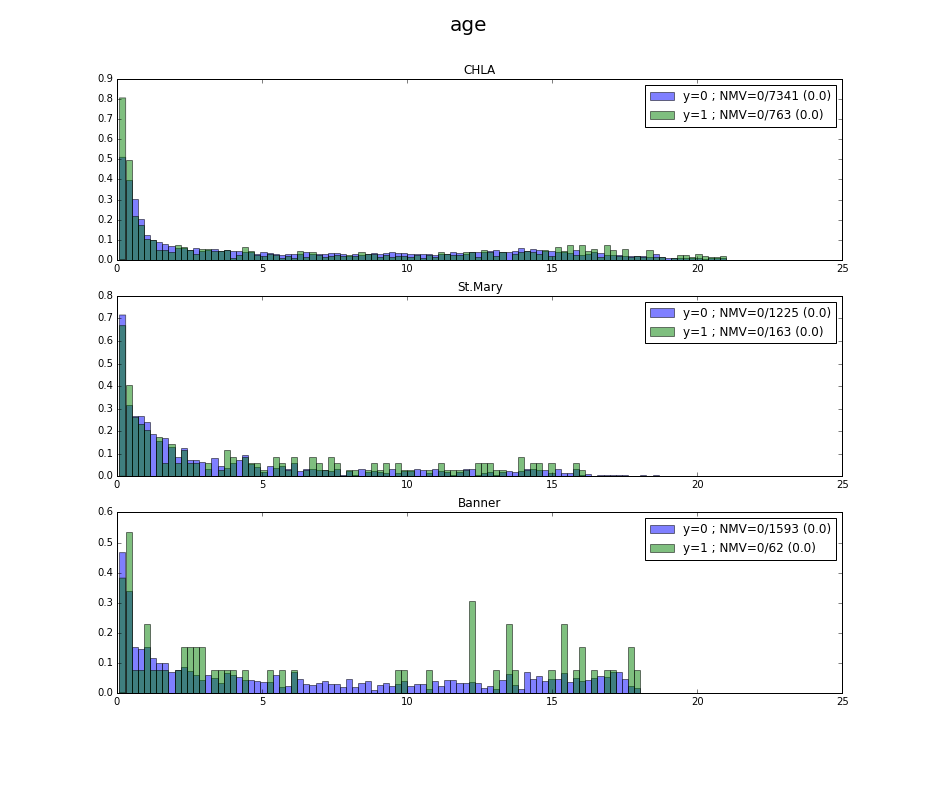
\includegraphics[width=\textwidth]{./figures/age.png}
%\caption{Age distribution for the AKI and stable groups (y-axis corresponds to the number of encounters divided by the total number of encounters within each group, and x-axis corresponds to age in years) in three hospitals. Pruple bars correspond to AKI encounters and green bars correspond to stable encounters.} 
%\label{fig:age_dist}      
%\end{figure}


%\begin{figure}[!htbp]
%\centering
%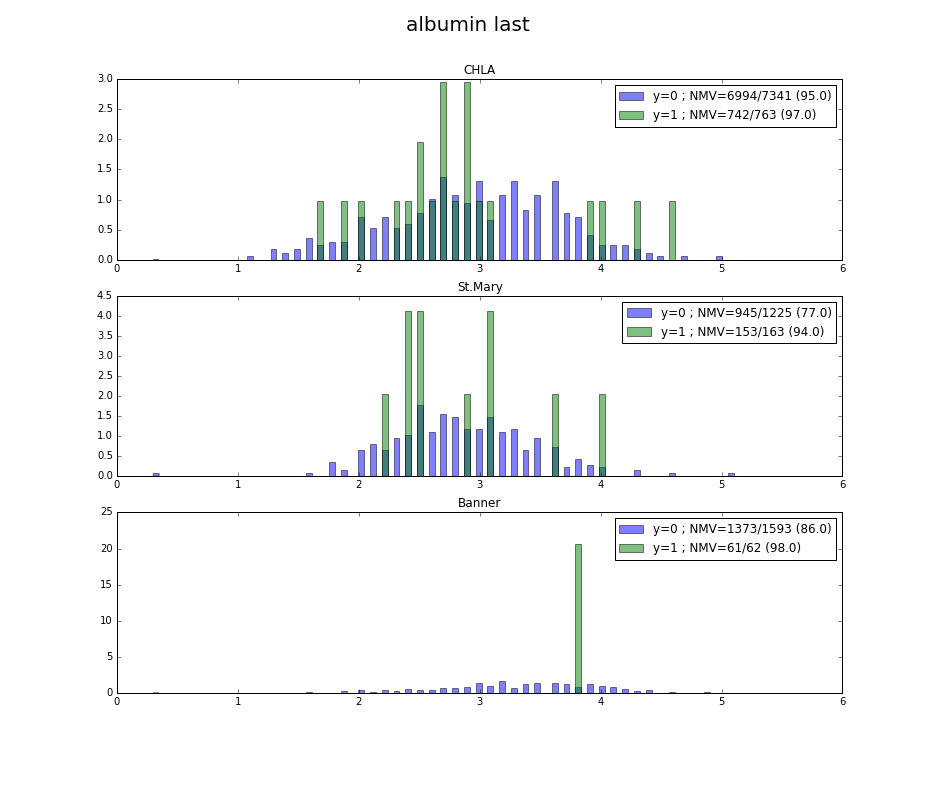
\includegraphics[width=\textwidth]{./figures/albumin_last.png}
%\caption{Albumin distribution for the AKI and stable groups (y-axis corresponds to the number of encounters divided by the total number of encounters within each group, and x-axis corresponds to albumin in g/dL)  in three hospitals. Pruple bars correspond to AKI encounters and green bars correspond to stable encounters.} 
%\label{fig:albumin_dist}      
%\end{figure}

\begin{figure}[!htbp]
\centering
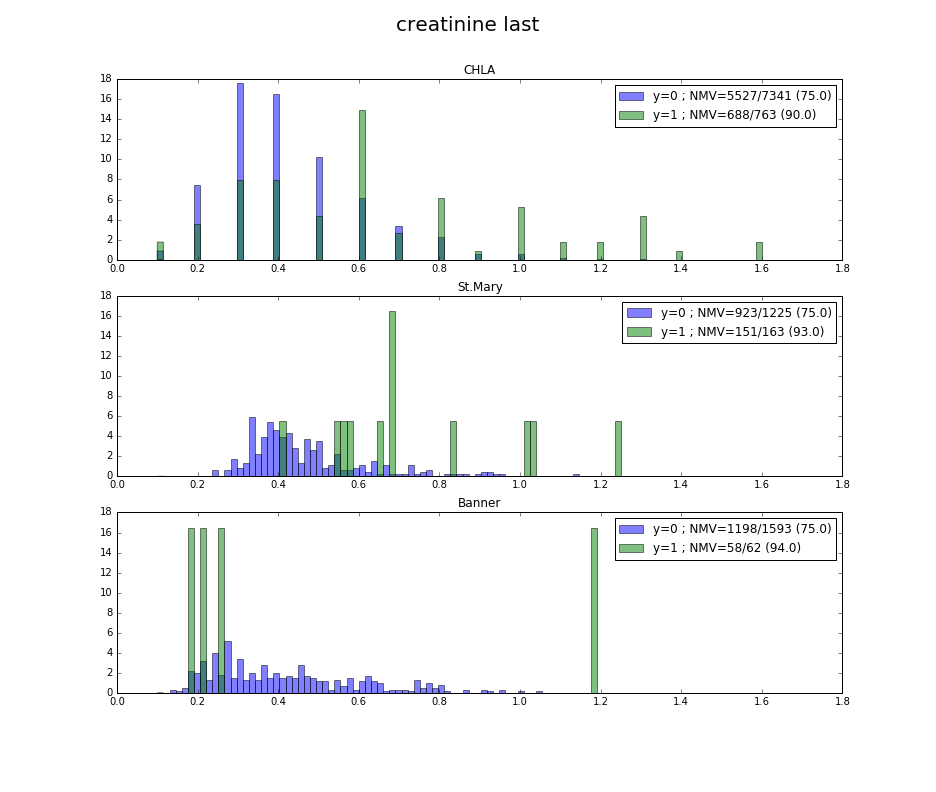
\includegraphics[width=\textwidth]{./figures/creatinine_last.png}
\caption{Creatinine distribution for the AKI and stable groups (y-axis corresponds to the number of encounters divided by the total number of encounters within each group, and x-axis corresponds to creatinine in mg/dL) in three hospitals. Pruple bars correspond to AKI encounters and green bars correspond to stable encounters.} 
\label{fig:creatinine_dist}      
\end{figure}


%\begin{figure}[!htbp]
%\centering
%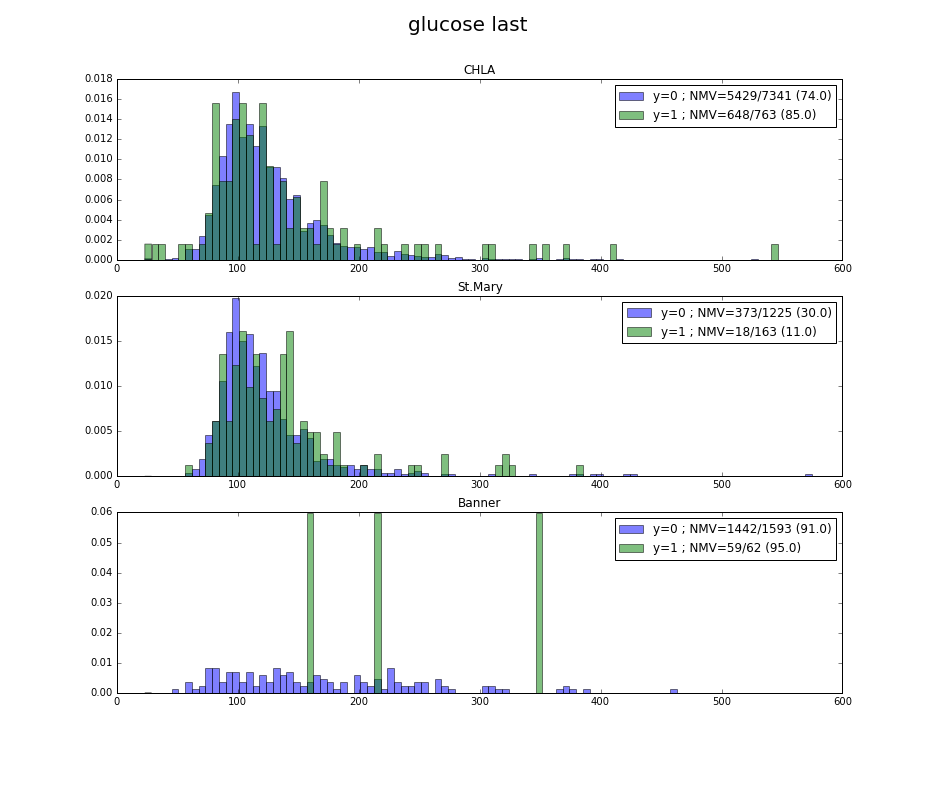
\includegraphics[width=\textwidth]{./figures/glucose_last.png}
%\caption{Glucose distribution for the AKI and stable groups (y-axis corresponds to the number of encounters divided by the total number of encounters within each group, and x-axis corresponds to glucose in mg/dL) in three hospitals. Pruple bars correspond to AKI encounters and green bars correspond to stable encounters.} 
%\label{fig:glucose_dist}      
%\end{figure}

%\begin{figure}[!htbp]
%\centering
%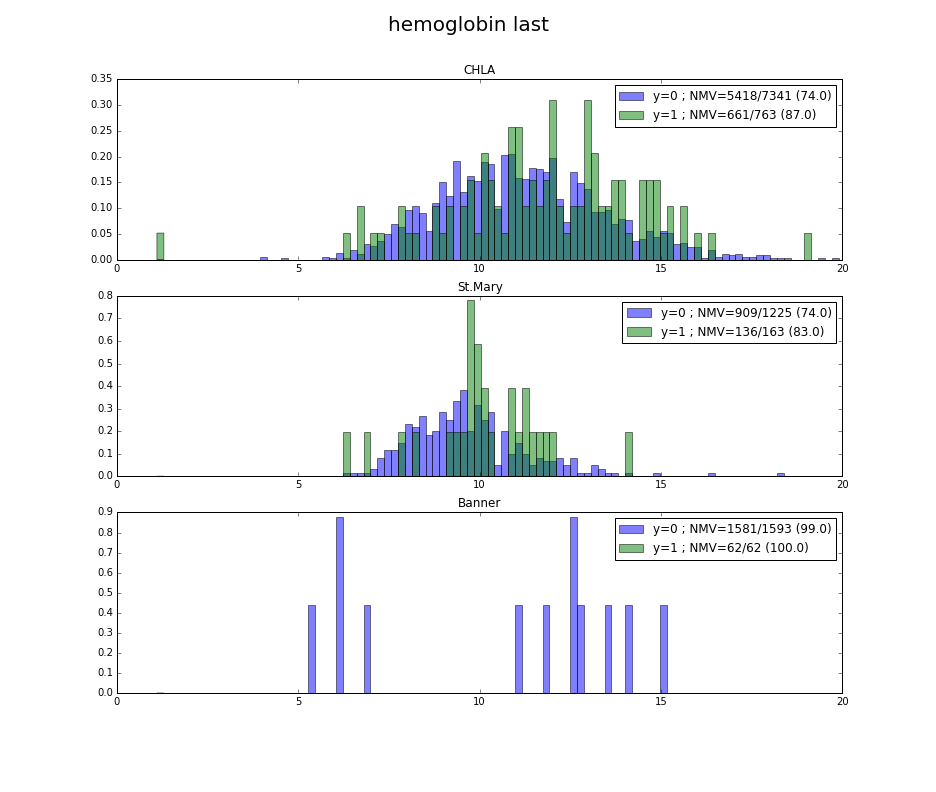
\includegraphics[width=\textwidth]{./figures/hemoglobin_last.png}
%\caption{Hemoglobin distribution for the AKI and stable groups (y-axis corresponds to the number of encounters divided by the total number of encounters within each group, and x-axis corresponds to hemoglobin in g/dL) in three hospitals. Pruple bars correspond to AKI encounters and green bars correspond to stable encounters.} 
%\label{fig:hemoglobin_dist}      
%\end{figure}

%\begin{figure}[!htbp]
%\centering
%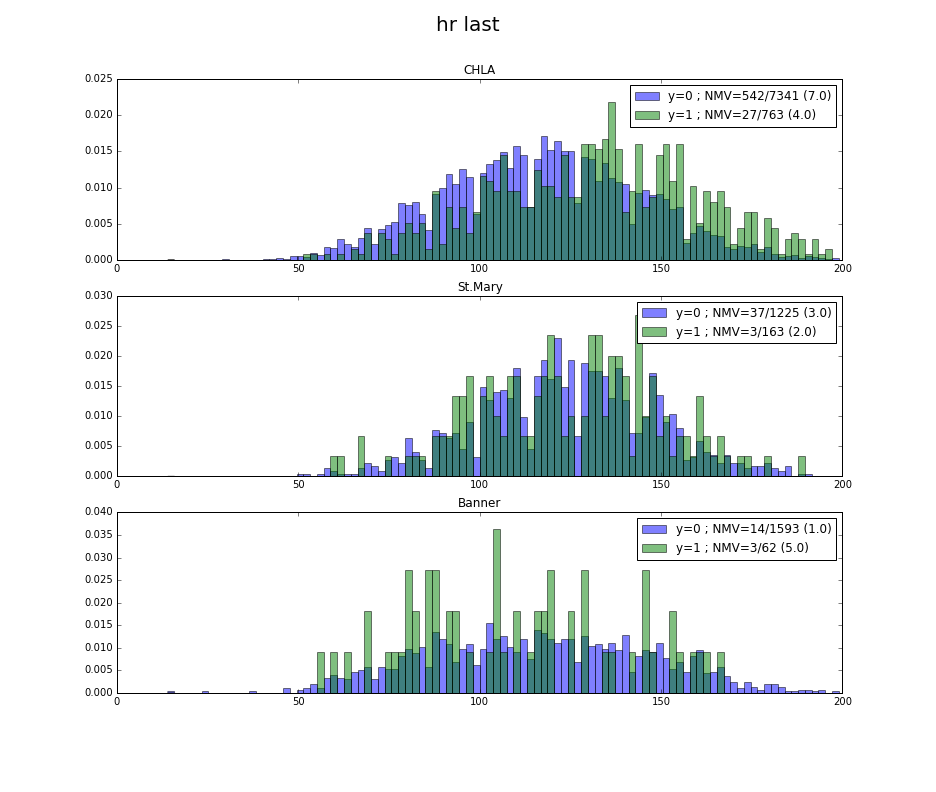
\includegraphics[width=\textwidth]{./figures/hr_last.png}
%\caption{Heart rate distribution for the AKI and stable groups (y-axis corresponds to the number of encounters divided by the total number of encounters within each group, and x-axis corresponds to heart rate in bpm) in three hospitals. Pruple bars correspond to AKI encounters and green bars correspond to stable encounters.} 
%\label{fig:hr_dist}      
%\end{figure}

%\begin{figure}[!htbp]
%\centering
%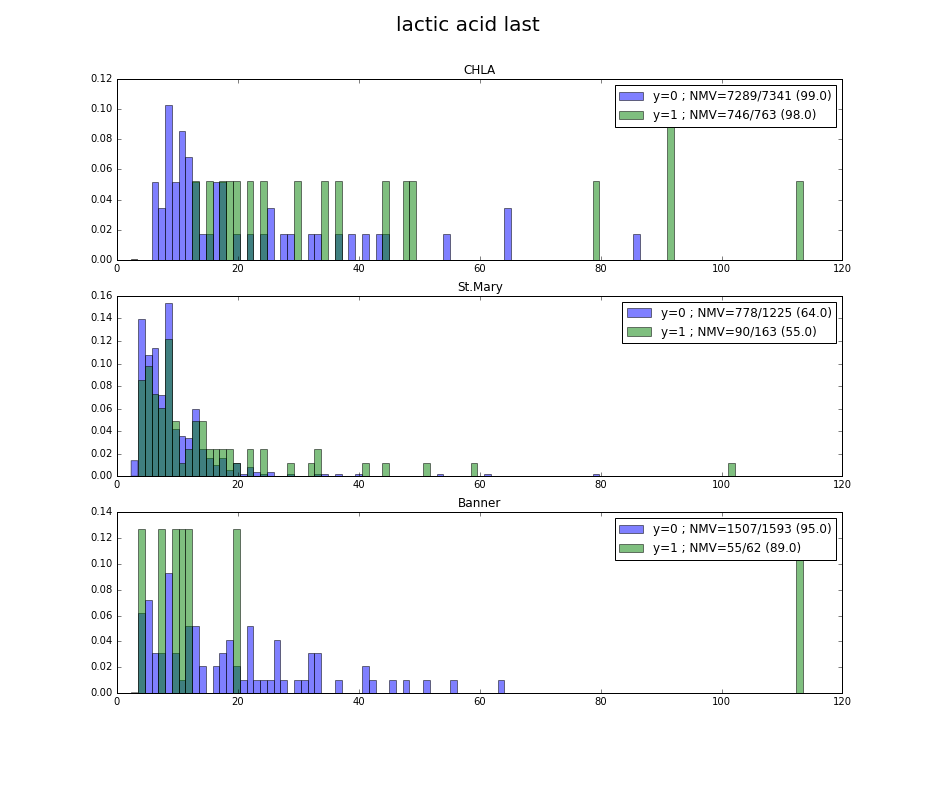
\includegraphics[width=\textwidth]{./figures/lactic_acid_last.png}
%\caption{Lactic acid distribution for the AKI and stable groups (y-axis corresponds to the number of encounters divided by the total number of encounters within each group, and x-axis corresponds to lactic acid in mg/dL) in three hospitals. Pruple bars correspond to AKI encounters and green bars correspond to stable encounters.} 
%\label{fig:lactic_acid_dist}      
%\end{figure}

\begin{figure}[!htbp]
\centering
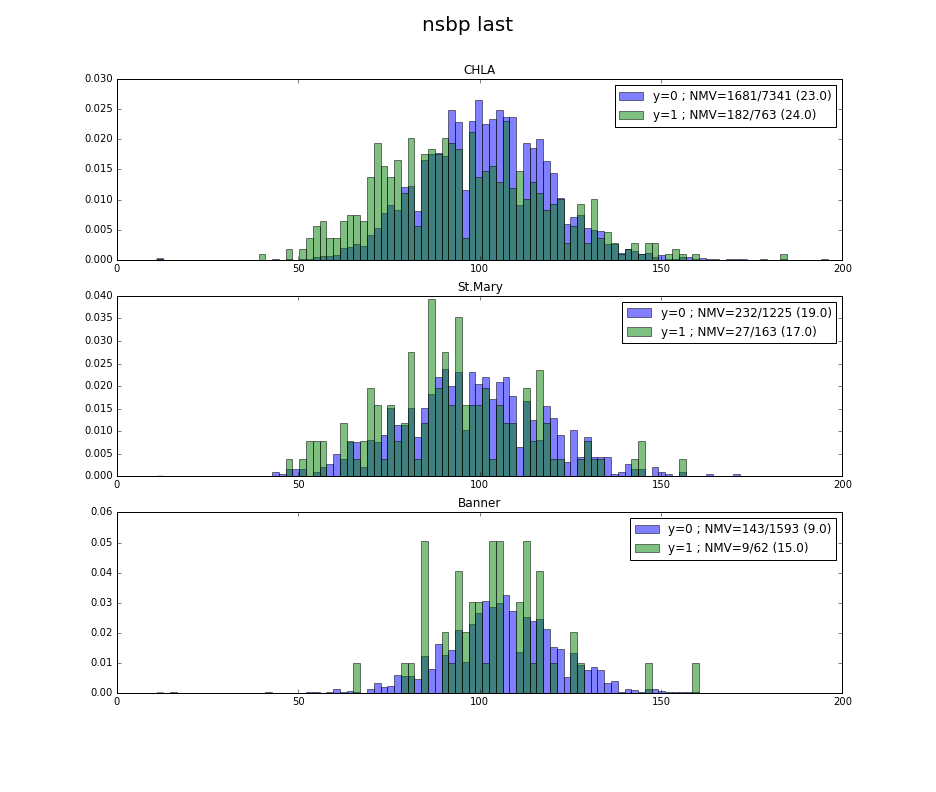
\includegraphics[width=\textwidth]{./figures/nsbp_last.png}
\caption{Non-invasive Systolic Blood Pressure (nSBP) distribution for the AKI and stable groups (y-axis corresponds to the number of encounters divided by the total number of encounters within each group, and x-axis corresponds to nSBP in mmHg) in three hospitals. Pruple bars correspond to AKI encounters and green bars correspond to stable encounters.} 
\label{fig:nsbp_dist}      
\end{figure}

%\begin{figure}[!htbp]
%\centering
%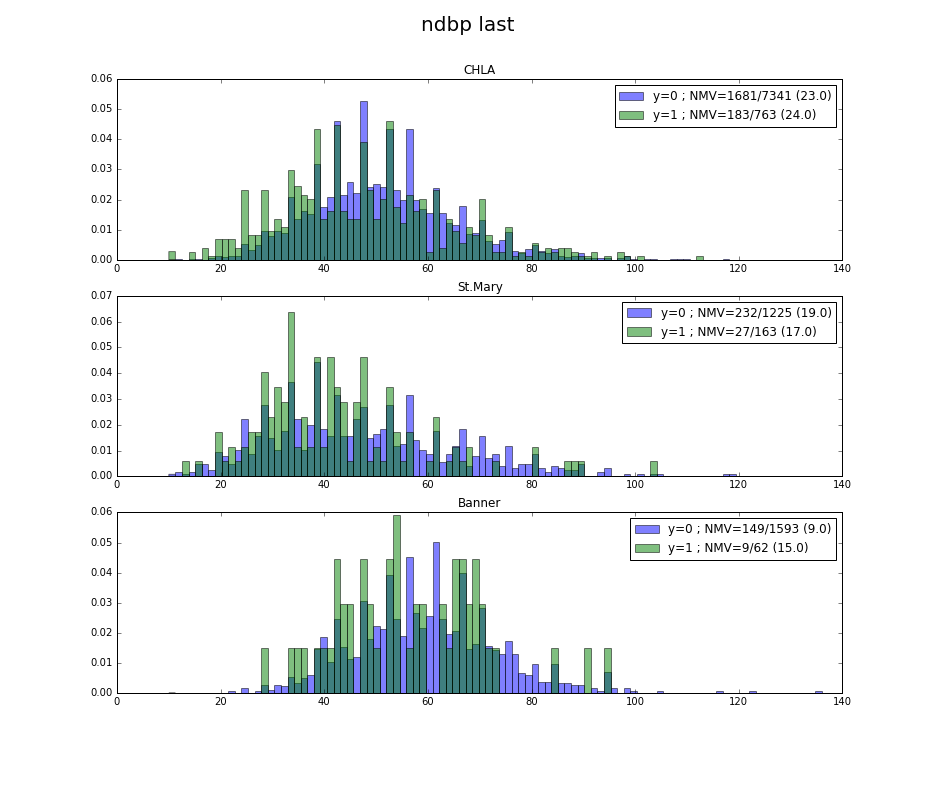
\includegraphics[width=\textwidth]{./figures/ndbp_last.png}
%\caption{Non-invasive Diastolic Blood Pressure (nDBP) distribution for the AKI and stable groups (y-axis corresponds to the number of encounters divided by the total number of encounters within each group, and x-axis corresponds to nDBP in mmHg) in three hospitals. Pruple bars correspond to AKI encounters and green bars correspond to stable encounters.} 
%\label{fig:ndbp_dist}      
%\end{figure}

%\begin{figure}[!htbp]
%\centering
%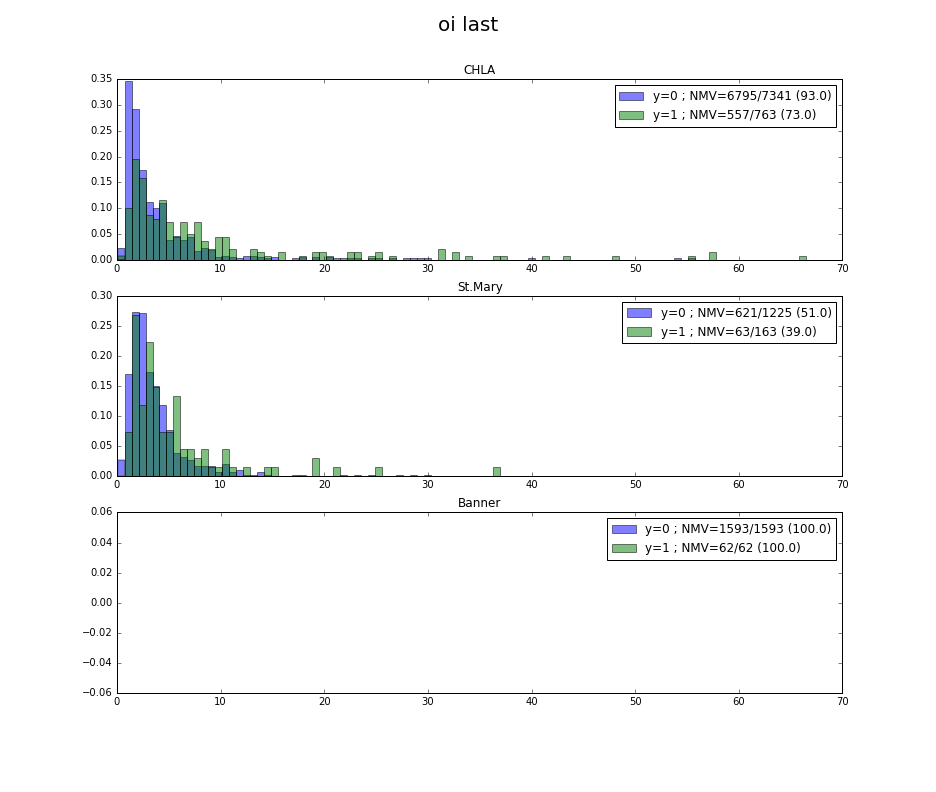
\includegraphics[width=\textwidth]{./figures/oi_last.png}
%\caption{Oxygenation Index (OI) distribution for the AKI and stable groups (y-axis corresponds to the number of encounters divided by the total number of encounters within each group, and x-axis corresponds to OI) in three hospitals. Pruple bars correspond to AKI encounters and green bars correspond to stable encounters.} 
%\label{fig:oi_dist}      
%\end{figure}

\begin{figure}[!htbp]
\centering
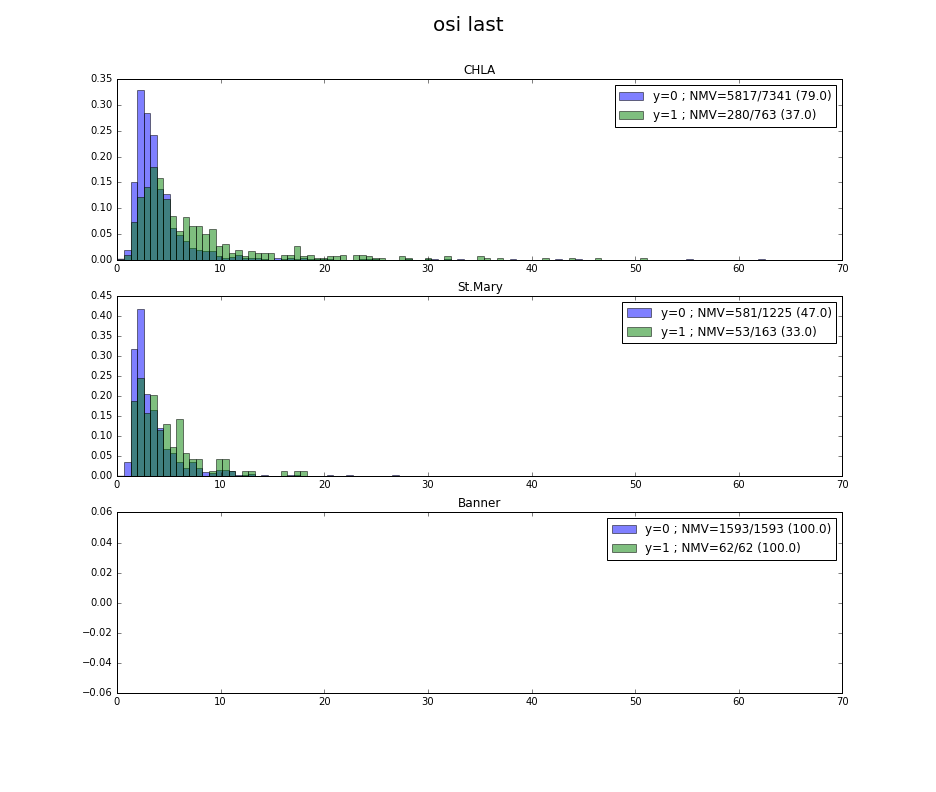
\includegraphics[width=\textwidth]{./figures/osi_last.png}
\caption{Oxygen Saturation Index (OSI) distribution for the AKI and stable groups (y-axis corresponds to the number of encounters divided by the total number of encounters within each group, and x-axis corresponds to OSI in $\text{cmH}_2\text{O}$) in three hospitals. Pruple bars correspond to AKI encounters and green bars correspond to stable encounters.} 
\label{fig:osi_dist}      
\end{figure}

\begin{figure}[!htbp]
\centering
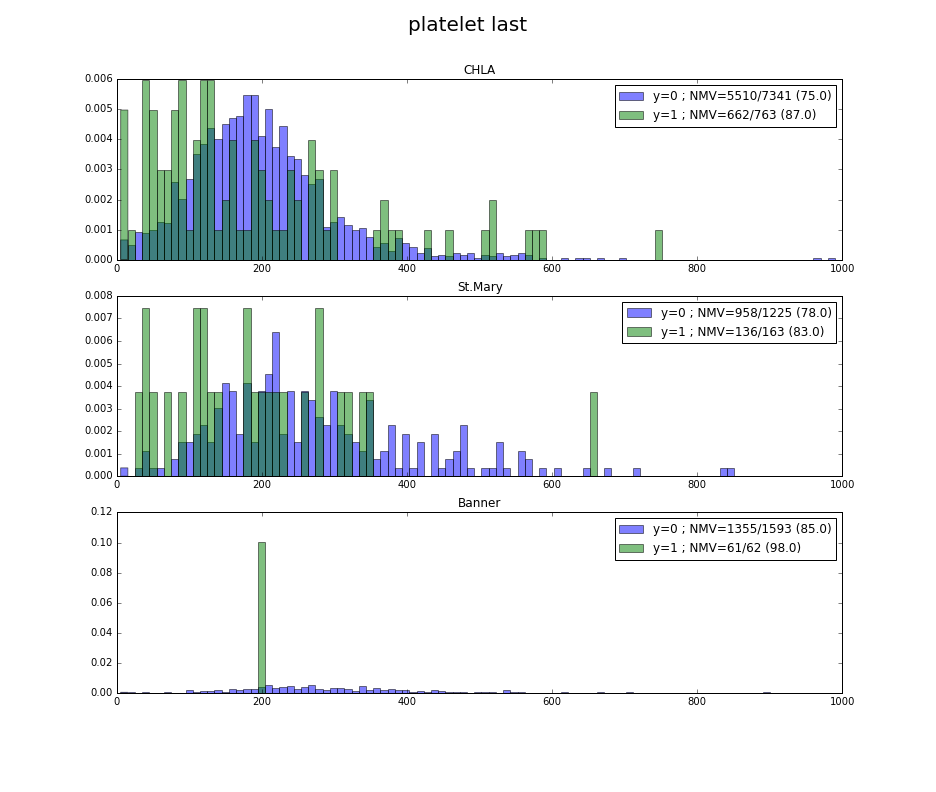
\includegraphics[width=\textwidth]{./figures/platelet_last.png}
\caption{Platelet count distribution for the AKI and stable groups (y-axis corresponds to the number of encounters divided by the total number of encounters within each group, and x-axis corresponds to platelet count in K/$\mu$L) in three hospitals. Pruple bars correspond to AKI encounters and green bars correspond to stable encounters.} 
\label{fig:platelet_dist}      
\end{figure}

%\begin{figure}[!htbp]
%\centering
%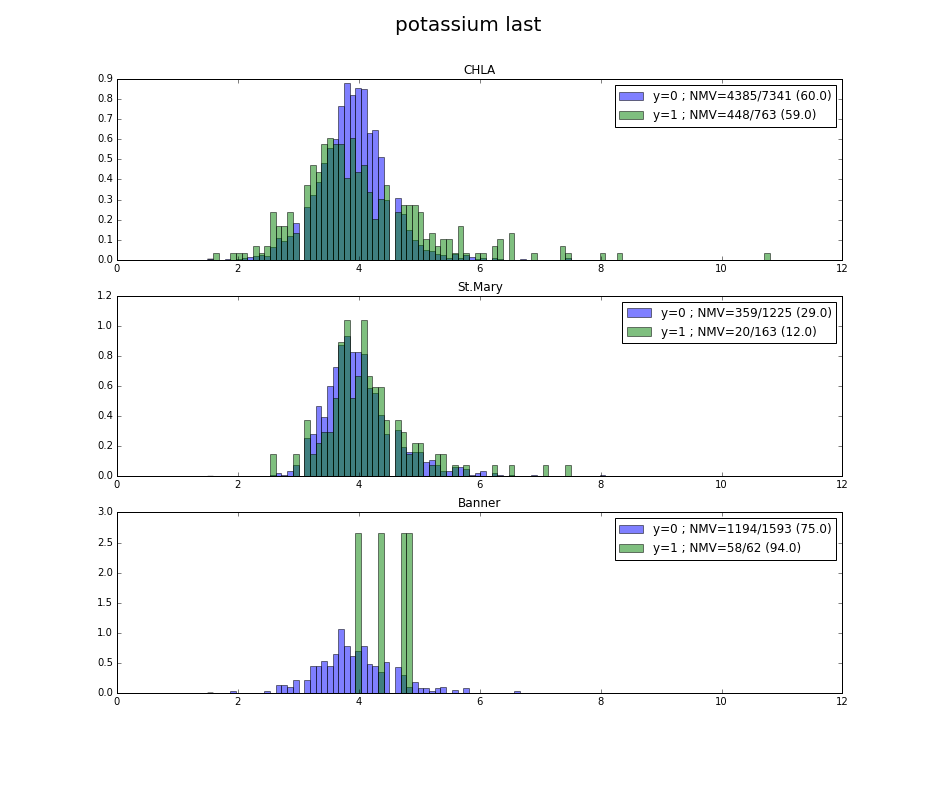
\includegraphics[width=\textwidth]{./figures/potassium_last.png}
%\caption{Potassium distribution for the AKI and stable groups (y-axis corresponds to the number of encounters divided by the total number of encounters within each group, and x-axis corresponds to potassium in meq/L) in three hospitals. Pruple bars correspond to AKI encounters and green bars correspond to stable encounters.} 
%\label{fig:potassium_dist}      
%\end{figure}

%\begin{figure}[!htbp]
%\centering
%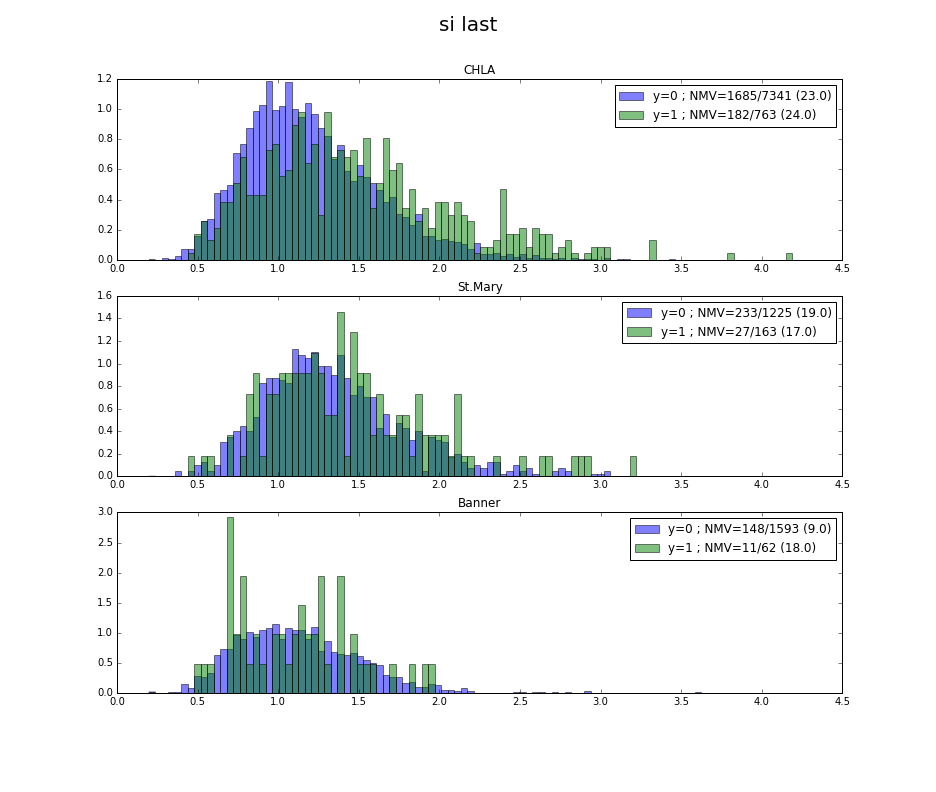
\includegraphics[width=\textwidth]{./figures/si_last.png}
%\caption{Shock Index (SI) distribution for the AKI and stable groups (y-axis corresponds to the number of encounters divided by the total number of encounters within each group, and x-axis corresponds to SI in bpm/mmHg) in three hospitals. Pruple bars correspond to AKI encounters and green bars correspond to stable encounters.} 
%\label{fig:si_dist}      
%\end{figure}

%\begin{figure}[!htbp]
%\centering
%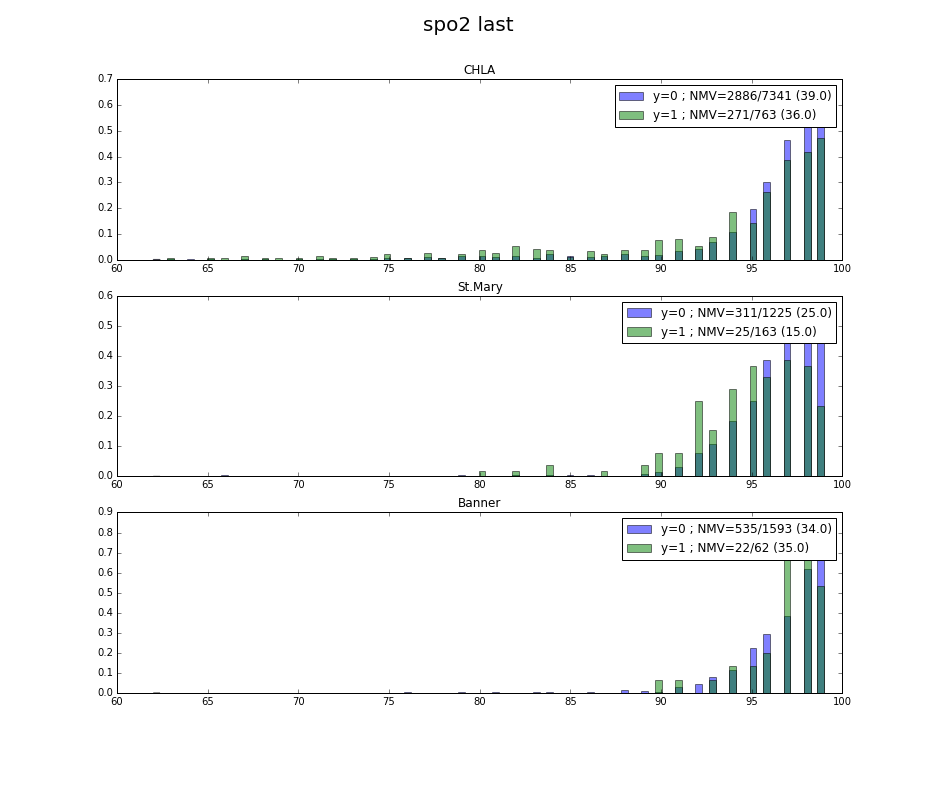
\includegraphics[width=\textwidth]{./figures/spo2_last.png}
%\caption{$\text{SpO}_2$ distribution for the AKI and stable groups (y-axis corresponds to the number of encounters divided by the total number of encounters within each group, and x-axis corresponds to $\text{SpO}_2$ in \%) in three hospitals. Pruple bars correspond to AKI encounters and green bars correspond to stable encounters.} 
%\label{fig:spo2_dist}      
%\end{figure}

%\begin{figure}[!htbp]
%\centering
%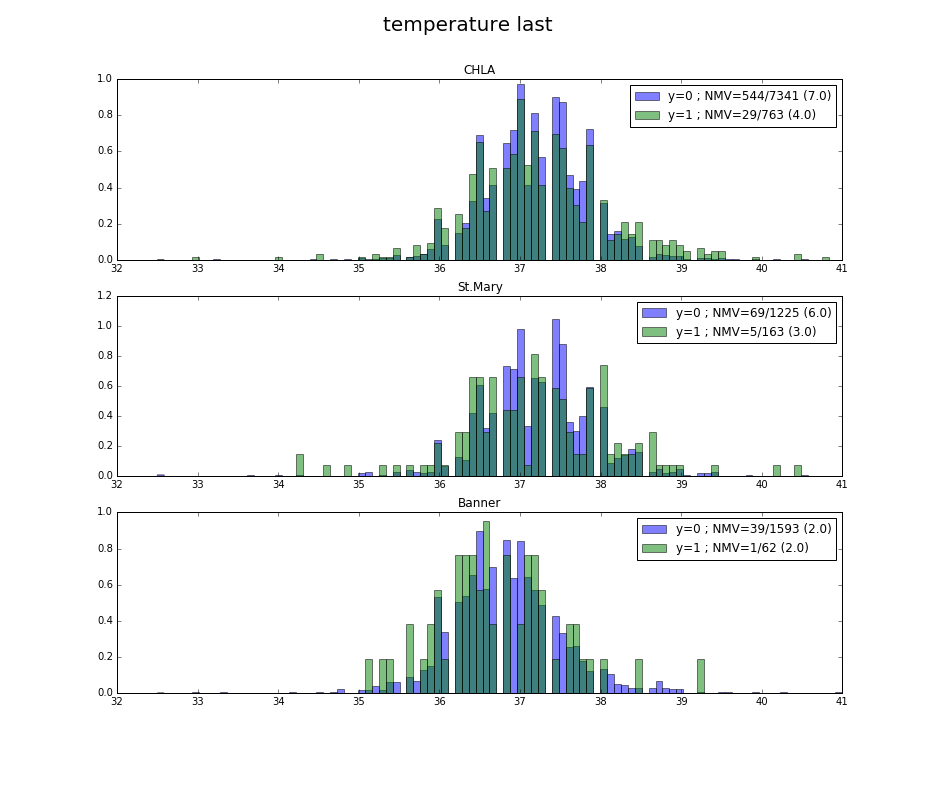
\includegraphics[width=\textwidth]{./figures/temperature_last.png}
%\caption{Temperature distribution for the AKI and stable groups (y-axis corresponds to the number of encounters divided by the total number of encounters within each group, and x-axis corresponds to temperature in $^{\circ}$C) in three hospitals. Pruple bars correspond to AKI encounters and green bars correspond to stable encounters.} 
%\label{fig:temperature_dist}      
%\end{figure}

%\begin{figure}[!htbp]
%\centering
%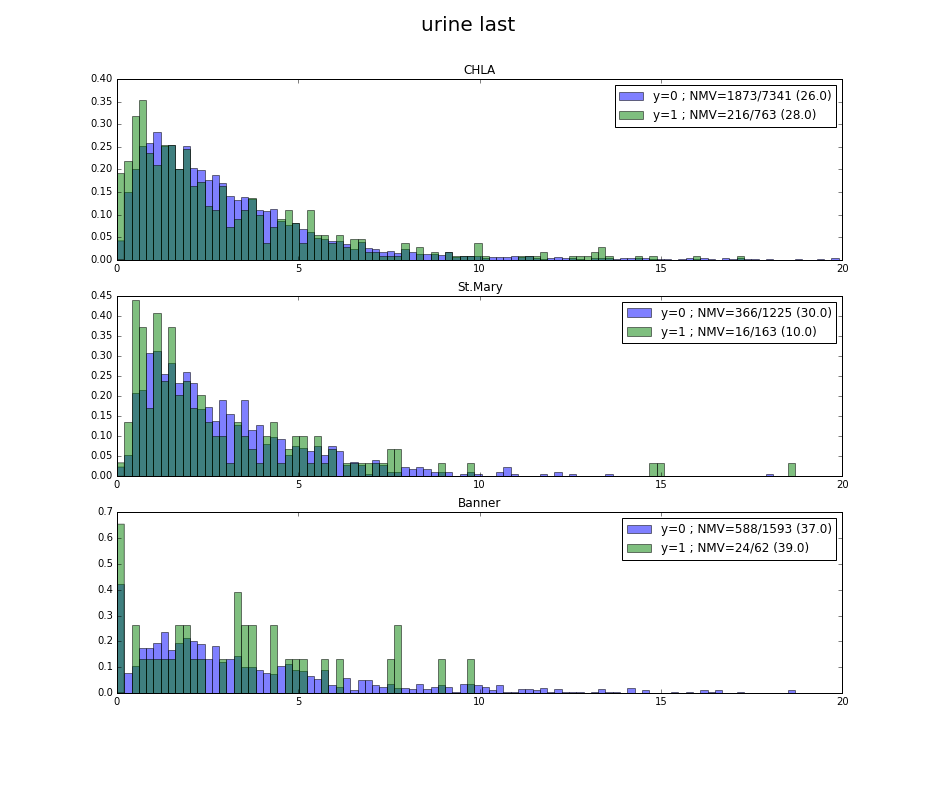
\includegraphics[width=\textwidth]{./figures/urine_last.png}
%\caption{Urine output distribution for the AKI and stable groups (y-axis corresponds to the number of encounters divided by the total number of encounters within each group, and x-axis corresponds to urine output in cc/kg/hr) in three hospitals. Pruple bars correspond to AKI encounters and green bars correspond to stable encounters.} 
%\label{fig:urine_dist}      
%\end{figure}

%\begin{figure}[!htbp]
%\centering
%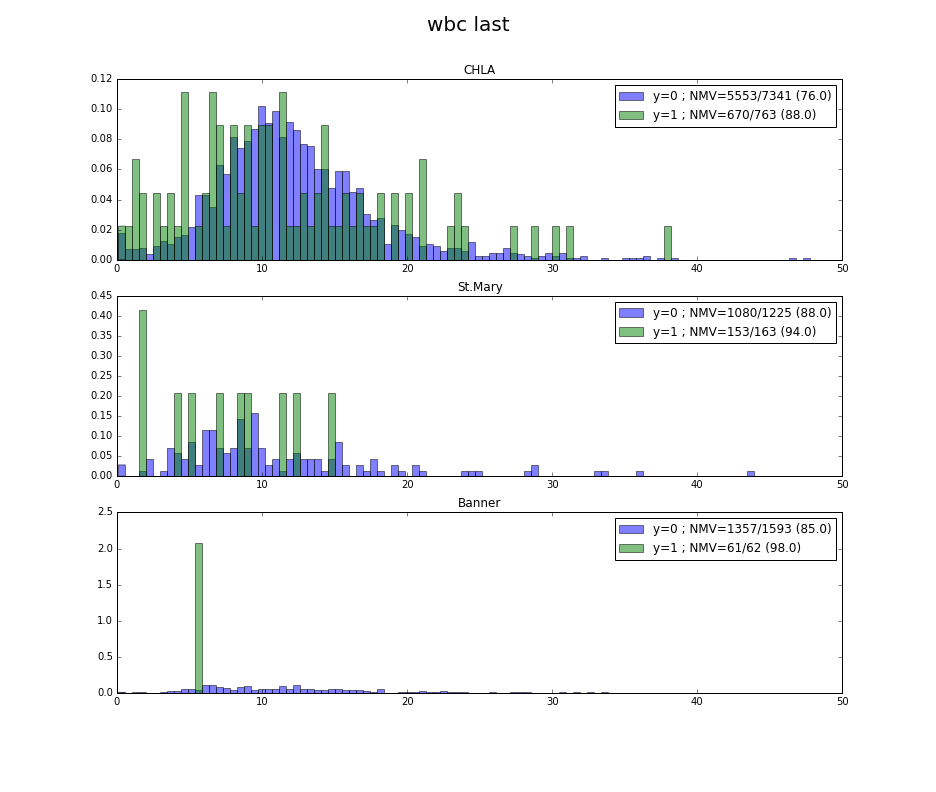
\includegraphics[width=\textwidth]{./figures/wbc_last.png}
%\caption{WBC count distribution for the AKI and stable groups (y-axis corresponds to the number of encounters divided by the total number of encounters within each group, and x-axis corresponds to WBC count in K/$\mu$ L) in three hospitals. Pruple bars correspond to AKI encounters and green bars correspond to stable encounters.} 
%\label{fig:wbc_dist}      
%\end{figure}

\section{Algorithm}

\subsection{Imputation of missing values}
%\subsubsection{Imputation by sample mean}
The mean of $j^{th}$ feature is computed using the examples where $j^{th}$ feature  is observed (\eq{}\ref{eqn:mean_value} assumes there are $M$ observed examples). Population mean value for $j^{th}$ feature is then used as the value for $j^{th}$ feature in examples where $j^{th}$ feature is not observed. A single completion of the data set is formed by imputing exactly one value for each unobserved feature. 

\begin{eqnarray}
\label{eqn:mean_value}
\bar{x_{j}} = \frac{1}{M}\sum_{k=1}^M x_{j}^{(k)}
\end{eqnarray}  

%\subsubsection{Imputation by estimated probability distribution}


\subsection{AdaBoost-abstain}
\label{sec:adaboost}
AdaBoost \cite{Schapire:1999} is a very effective machine learning technique for building a powerful classifier from an ensemble of ``weak learners''.  Specifically, the boosted classifier $H(\bm{x})$ is modeled as a generalized additive model of many base hypotheses:
\begin{eqnarray}
H(\bm{x}) = b + \sum_{t} \alpha_t h(\bm{x}; \bm{\theta_t})
\label{eqn:additive}
\end{eqnarray}
where $b$ is a constant bias that accounts for the prevalence of the categories, and each $h(\bm{x};\bm{\theta_t})$ is a function of $\bm{x}$, with parameters given by the elements in the vector $\bm{\theta_t}$, and produces a classification output ($+1$ or $-1$).  We also allow each of the base classifiers to abstain from voting (output=$0$).  A final classification decision is assigned by taking the sign of $H(\bm{x})$, which results in a weighted majority vote over the base classifiers in the model.

As is common for AdaBoost applications, we use the class of 1-dimensional decision stumps as the base hypotheses:
\begin{equation}
h(\bm{x}; \bm{\theta_t}=(j,\tau)) = \left\{\begin{array}{rl} +1\text{, } & x_j \geq \tau \\ -1\text{, } & x_j < \tau \\ 0\text{, } & x_j = \phi \\ \end{array}\right.
\end{equation}
Thus, each base classifier votes by comparing one of the $p$ features in the data to a threshold.  If that particular feature is missing, the base classifier abstains from voting.

The algorithm to learn the bias $b$, base hypotheses $h(\bm{x};\bm{\theta_t})$ and weightings $\alpha_t$ is a version of the traditional discrete AdaBoost algorithm adapted to accommodate classifiers that abstain, which was described in \cite{Schapire:1999}. This algorithm has been employed previously for missing data problems in predicting protein-protein interactions \cite{Smeraldi:2010}, but since it is a non-standard application of AdaBoost, we briefly reproduce the details of the algorithm here.

AdaBoost seeks to minimize the exponential loss function:
\begin{eqnarray}
L = \sum_{i=1}^n \exp\left(-y^{(i)} H(\bm{x^{(i)}})\right)
\label{eqn:adaboost_exp_loss}
\end{eqnarray}
which can be shown to be an upper bound on the training error \cite{Freund:2009}.  Optimization proceeds in a greedy fashion: at each iteration (or boosting round) $t$, a new classifier is added to the model that most decreases the objective function in (\ref{eqn:adaboost_exp_loss}).  Thus, at iteration $t=T$, we fix the base classifiers learned at iterations $1,\dots,T-1$ and add a new classifier $h(\bm{x}; \bm{\theta_T})$, weighted by $\alpha_T$, that minimizes the exponential loss objective:
\begin{eqnarray}
\sum_{i=1}^n \exp\left(-y^{(i)}\left[b + \sum_{t=1}^{T-1} \alpha_t h(\bm{x^{(i)}}; \bm{\theta_t}) + \alpha_{T} h(\bm{x^{(i)}}; \bm{\theta_T})\right]\right) \\
= \sum_{i=1}^n w_i^{(T)} \exp\left(-y^{(i)} \alpha_T h(\bm{x^{(i)}}; \bm{\theta_T})\right) \label{eqn:adaboost_T}
\end{eqnarray}
where $w_1^{(T)},w_2^{(T)},\dots,w_n^{(T)}$ is the current weight distribution on the training data:
\begin{equation}
w_i^{(T)} = \exp\left(-y^{(i)}\left[b + \sum_{t=1}^{T-1} \alpha_t h(\bm{x^{(i)}}; \bm{\theta_t})\right]\right)
\end{equation}
These weights reflect how well the current classifier (up to iteration $T-1$) is performing on each of the training examples:  the larger the weight, the poorer the classifier predicts the true label of that example.

The algorithm boils down to selecting $h(\bm{x^{(i)}}; \bm{\theta_T})$ and $\alpha_T$.  It can be shown \cite{Schapire:1999} that the classifier that most decreases the objective is the one that minimizes:
\begin{eqnarray}
D_0(\bm{\theta_T}) &+& 2\sqrt{D_{+}(\bm{\theta_T})D_{-}(\bm{\theta_T})} \label{eqn:clf_selection_criterion} \\ 
\text{where} & & D_0(\bm{\theta_T}) = \sum_{i=1}^n w_i^{(T)} \mathbb{I}(h(\bm{x^{(i)}};\bm{\theta_T}) = 0) \\
			 & & D_{+}(\bm{\theta_T}) = \sum_{i=1}^n w_i^{(T)} \mathbb{I}(y^{(i)}h(\bm{x^{(i)}};\bm{\theta_T}) > 0) \\
			 & & D_{-}(\bm{\theta_T}) = \sum_{i=1}^n w_i^{(T)} \mathbb{I}(y^{(i)}h(\bm{x^{(i)}};\bm{\theta_T}) < 0) \\
\end{eqnarray}
where $\mathbb{I}(x)$ is the indicator function.  Intuitively, $D_0(\bm{\theta_T})$, $D_{+}(\bm{\theta_T})$ and $D_{-}(\bm{\theta_T})$ are the fraction of examples (under the current training weight distribution) for which the classifier abstains, classifies correctly, and classifies incorrectly.
This best classifier can be identified efficiently from the class of decision stumps.

Once the classifier has been selected, the weight can be computed analytically by setting the derivative of (\ref{eqn:adaboost_T}) to zero, resulting in the following update:
\begin{equation}
\alpha_T = \frac{1}{2} \log\left(\frac{D_{+}(\bm{\theta_T})}{D_{-}(\bm{\theta_T})}\right)
\end{equation}
Notice that even though the classifier selection criterion (\ref{eqn:clf_selection_criterion}) penalizes a classifier for abstaining, the weighting $\alpha_T$ that it is assigned if it is selected is not affected.  Instead, a classifier's weighting only depends on how discriminative it is when it votes, and is not penalized for abstaining.

Upon incorporating the weighted classifier $\alpha_Th(\bm{x};\bm{\theta_T})$, we update the weight distribution:
\begin{equation}
w_i^{(T+1)} \gets w_i^{(T)} \exp\left(-y^{(i)} \alpha_T h(\bm{x^{(i)}};\bm{\theta_T})\right)
\end{equation}
and proceed to the next round of boosting $t=T+1$.

If the prevalence of hemodynamic instability in the ICU dataset is unbalanced, the best classifier to add may often be one that is highly biased towards the most prevalent category.  To remove this effect, we re-tune the bias at each iteration.  Specifically, at the start of each boosting round, the bias is adjusted as follows:

\begin{eqnarray}
b &\gets& b + \Delta_b \\
\Delta_b &=& \frac{1}{2}\log\left(\frac{\sum_{i=1}^n w_i^{(T)} \mathbb{I}(y^{(i)} = +1)}{\sum_{i=1}^n w_i^{(T)} \mathbb{I}(y^{(i)} = -1)}\right) \end{eqnarray}
This update adjusts the weight distribution to:
\begin{equation}
w_i^{(T)} \gets w_i^{(T)}\exp(-y^{(i)}\Delta_b)
\end{equation}
which has the appealing property of equalizing the weight distribution on positively and negatively labeled examples:
\begin{equation}
\sum_{i=1}^n w_i^{(T)} \mathbb{I}(y^{(i)} = -1) = \sum_{i=1}^n w_i^{(T)} \mathbb{I}(y^{(i)} = +1)
\end{equation}
This removes the prevalence bias and forces the learning algorithm to select a classifier with good separation between the two classes.

To account for age-dependent clinical features, we introduced a slight modification in the algorithm. After a classifier has been selected at iteration $t$, we computed an age-based decision threshold based on a number of age groups. We defined a total of $65$ age groups -- the first 3 groups were $[0-3)$,$[3-6)$ and $[6-12)$ months. The remaining age groups were defined from $1$ to $20$ years old, in steps of 1.5 years, and offset of 0.25 years (\eg{} $[1-2.5)$,$[1.25-2.75),\dots,[18.5-20))$. The notation $[a,b) = \left\{x \in \mathbb{R} \mid a\leq x<b \right\}$. If the selected weak learner depended on any of the following features:(nSI, iSI, nSBP, iSBP, nMBP, iMBP, nDBP, iDBP, HR, or PPA), a quadratic function was fitted to the decision thresholds; otherwise, a linear function was fitted. The weight $\alpha_T$ was recomputed by using a line search (\ie{} finding the root of the derivative of \eq{} \ref{eqn:adaboost_T} with respect to $\alpha_T$ as shown in \eq{} \ref{eqn:linesearch})

%The resulting $65$ decision thresholds were then smoothed with a median filter of order 4 (\ie{} median values across 4 consecutive age groups).

\begin{equation}
\label{eqn:linesearch}
\frac{\partial L}{\partial\alpha_{t}}= -\sum_{i=1}^n w_i^{(T)}y^{(i)} h\left(\bm{x^{(i)}},\text{age}; \bm{\theta_T}\right) \exp\left(-y^{(i)} \alpha_T h\left(\bm{x^{(i)}},\text{age}; \bm{\theta_T}\right)\right)
\end{equation}
%\exp\left(-y^{(i)} \alpha_T h(\bm{x^{(i)}}; \bm{\theta_T})\right

After $T$ rounds of boosting, we obtain a static ensemble classifier $H(\bm{x})$.  The set of bivariate classifiers $f_1(x_1,\text{age}),f_2(x_2,\text{age}),\dots,f_p(x_p,\text{age})$ that comprise this ensemble are the weighted sum of decision stumps acting on each of the features. So at the end of each boosting round $t=T$, if the selected base classifier operates on feature $x_j$, we update the appropriate bivariate classifier $f_j(x_j,\text{age}) \gets f_j(x_j,\text{age}) + \alpha_T h(\bm{x},\text{age};\bm{\theta_T})$.  Thus, $H(\bm{x})$ can be equivalently expressed as $H(\bm{x})=\sum_{j=1}^p f_j(x_j,\text{age})$. 


\subsection{Logistic Regression}
\label{sec:logreg}
Logistic regression predicts a binary response variable based on one or more predictor variables (features), which can be discrete and/or continuous. Specifically, logistic regression measures the relationship between the response variable and one or more independent variables by estimating probabilities using a logistic function. The linear logistic regression model takes the form shown in \eq{}\ref{eqn:logit}, where $\bm{w}$ is a p-dimensional vector referred to as the weight vector, and $b$ is the bias. The parameters $\bm{w}$ and $b$ can be estimated using maximum likelihood estimation.

\begin{eqnarray}
p(y_{i}=1 \mid \bm{x_{i}})=\frac{1}{1+\exp\left(-\left(\bm{w}^{T}\bm{x_{i}}+b\right)\right)} \label{eqn:logit}
\end{eqnarray}

\chapter{Results}
In this section, we show the analysis results for designing the algorithm. Only 18 features out of 111 features were included in the final algorithm since there was negligible performance drop by excluding the others. This is advantageous for algorithm deployment. Based on the 18 features included, AdaBoost-abstain algorithm showed better performance over logistic regression, therefore AdaBoost-abstain algorithm was chosen as the final algorithm. By cross validating the AdaBoost-abstain algorithm over different hospitals, we found that training the algorithm by data sets from different hospitals generalizes better among different hospitals and age groups.

\section{Comparison between AdaBoost-abstain and Logistic Regression}
\label{sec:lr_ab_compare} 
AdaBoost-abstain algorithm provided better AUC performance than logistic regression algorithm as shown in \fig \ref{fig:lrVSab}. Each algorithm was trained by the data set extracted from CHLA when the prediction window was 0 hour and observation window was 6 hours. Each trained algorithm was tested on data sets from either CHLA or St.Mary's hospital for prediction window ranging from 1 hour to 18 hours and observation window 6 hours. Dotted lines in the left figure shows Area Under the ROC curve (AUC) of the logistic regression model as a function of prediction window ranging from 1 hour to 18 hour. Solid lines in the right figure shows AUC of the Adaoost-abstain model as a function of prediction window ranging from 1 hour to 18 hour. For example, blue sold line shows the test AUC as a function of varying prediction window of the AdaBoost-abstain algorithm, where this algorithm was trained by CHLA data set at prediction window = 0 hour, and observation window = 6 hours. As the prediction window increases, tendency of dropping AUC was observed in all cases. Average test AUC over the 18 hour prediction window were 0.76 and 0.69 respectively for AdaBoost-abstain and logistic regression when the models were tested in CHLA data sets. Average test AUC of AdaBoost-abstain algorithm over prediction window from 1 hour to 18 hours dropped to 0.65 when it was tested in St.Mary's hospital. Similarly, for the logistic regression algorithm, average test AUC over prediction window from 1 hour to 18 hours dropped to 0.62. Since Adaboost-abstain algorithm showed better performance, Adaboost-abstain algorithm was exclusively considered in subsequent sections.

\begin{figure}[!htbp]
\centering
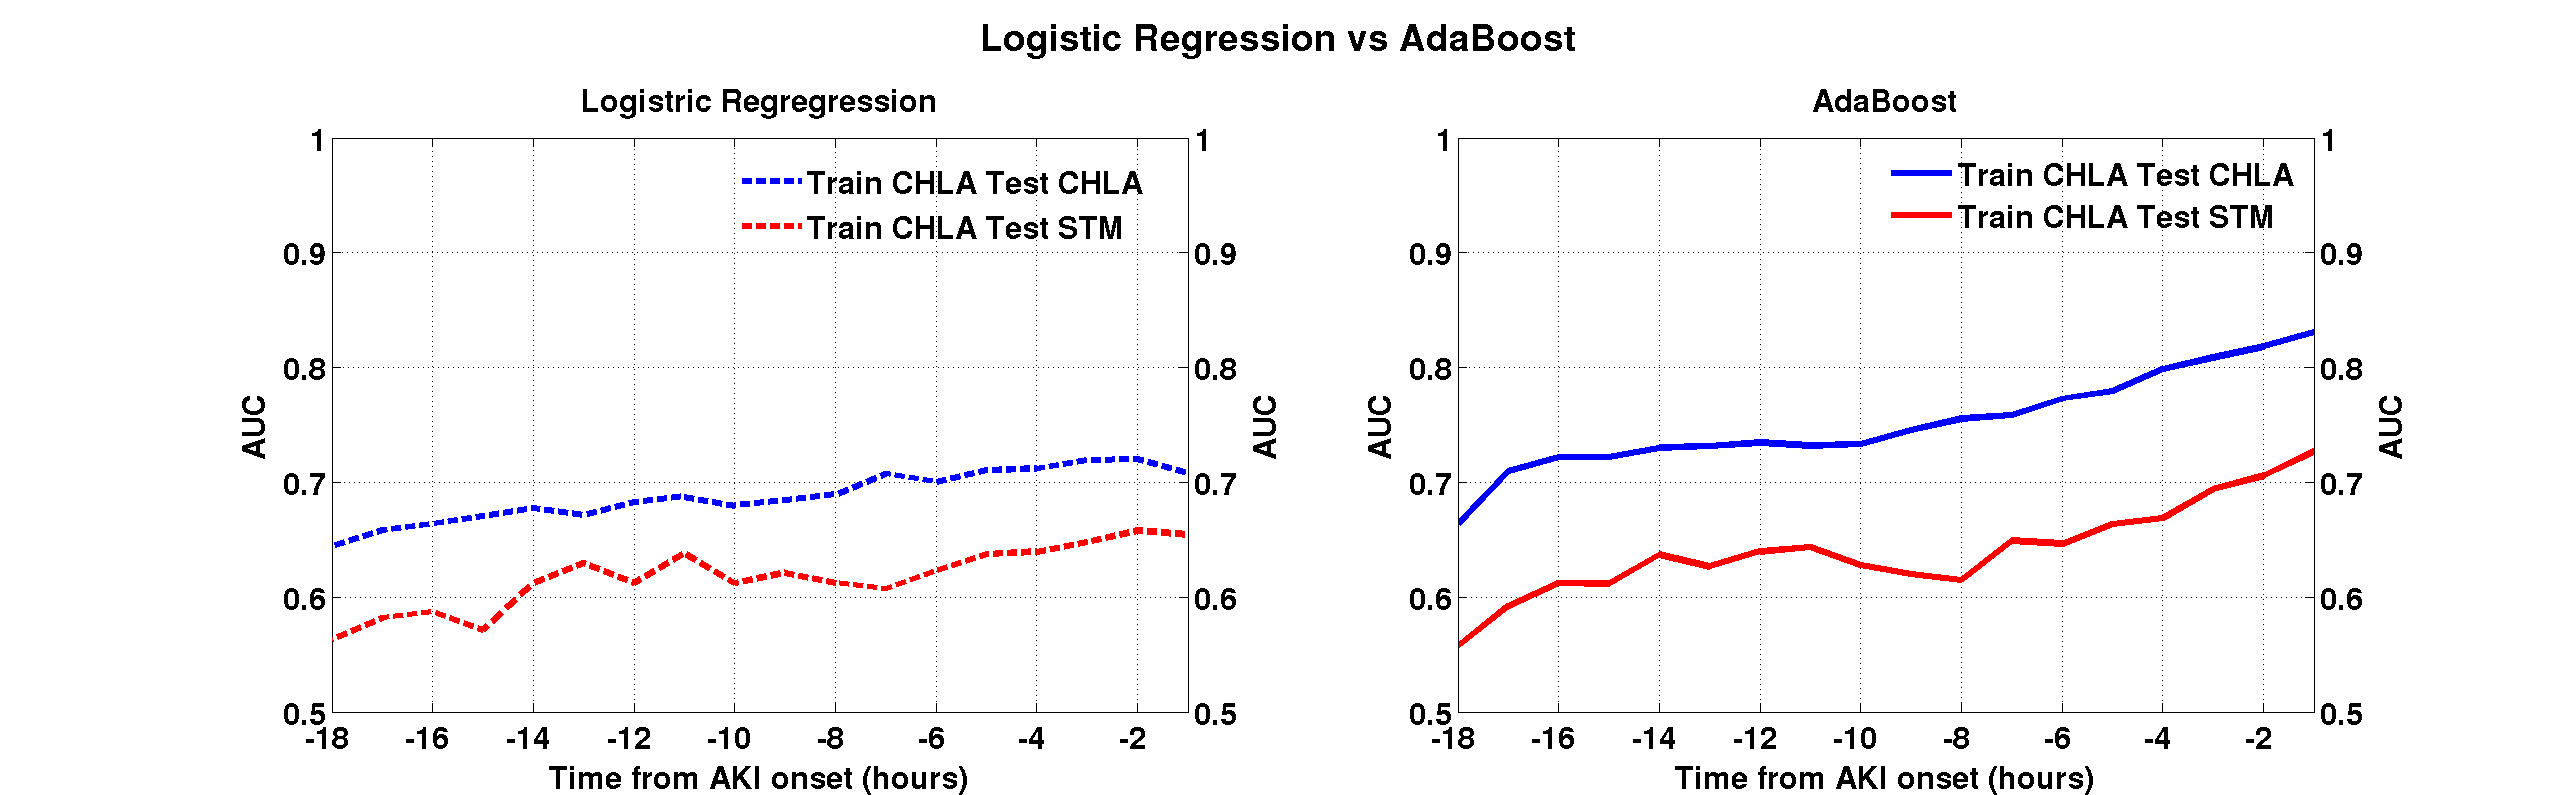
\includegraphics[width=\textwidth]{./figures/lrVSab_twin006.png}
\caption{Comparison between AdaBoost-abstain and logistic regression algorithms. Each algorithm was trained by the data set extracted from CHLA when the prediction window was 0 hour and observation window was 6 hours. Each trained algorithm was tested on data sets from either CHLA or St.Mary's hospital for prediction window ranging from 1 hour to 18 hours and observation window 6 hours. Dotted lines in the left figure shows AUC performance of the logistic regression model as a function of prediction window ranging from 1 hour to 18 hour. Solid lines in the right figure shows AUC performance of the Adaoost-abstain model as a function of prediction window ranging from 1 hour to 18 hour.} 
\label{fig:lrVSab}      
\end{figure}

\section{Cross Validation}
\label{sec:cv}
In this section, we cross validate the AdaBoost-abstain algorithm over different hospitals, CHLA and St.Mary's hospital. The Adaboost-Abstain algorithm was trained by three different data sets. First, the algorithm was trained by data set extracted from CHLA when prediction window was 0 hour and observation window was 6 hours. The second case was training the algorithm by a data set extracted from St.Mary's hospital when prediction window was 0 hour and observation window was 6 hours. The last case was training the algorithm by data sets extracted from CHLA and St.Mary's hospital when prediction window was 0 hour and observation windows was 6 hours. As shown in \fig{} \ref{fig:aucVStlag}, the solid lines corresponds to either the first or second case, and the dotted lines correspond to the last case. Blue and red solid lines show the cases when the model was trained and tested by data sets from a single hospital. These two lines are the AUC upper bounds of the AdaBoost-abstain algorithm, meaning that if the algorithm was trained by a combination of data sets from different hospitals then tested on each hospital, the test AUC on each hospital would be bounded by the test AUC of the algorithm trained by the single hospital. For example, the blue dotted line, which is the test AUC over CHLA data set of the algorithm was trained by a combined data from CHLA and St.Mary's hospital, shows lower values than the blue solid line. Black solid line shows the case when the algorithm was trained by CHLA data set and tested on St.Mary's hospital data sets. There is approximately 1 10\% AUC drop. However, the algorithm trained by a combination of two data sets from CHLA and St.Mary's shows less drop when tested on either hospitals as shown as the two dotted line in \fig{} \ref{fig:aucVStlag}.

\begin{figure}[!htbp]
\centering
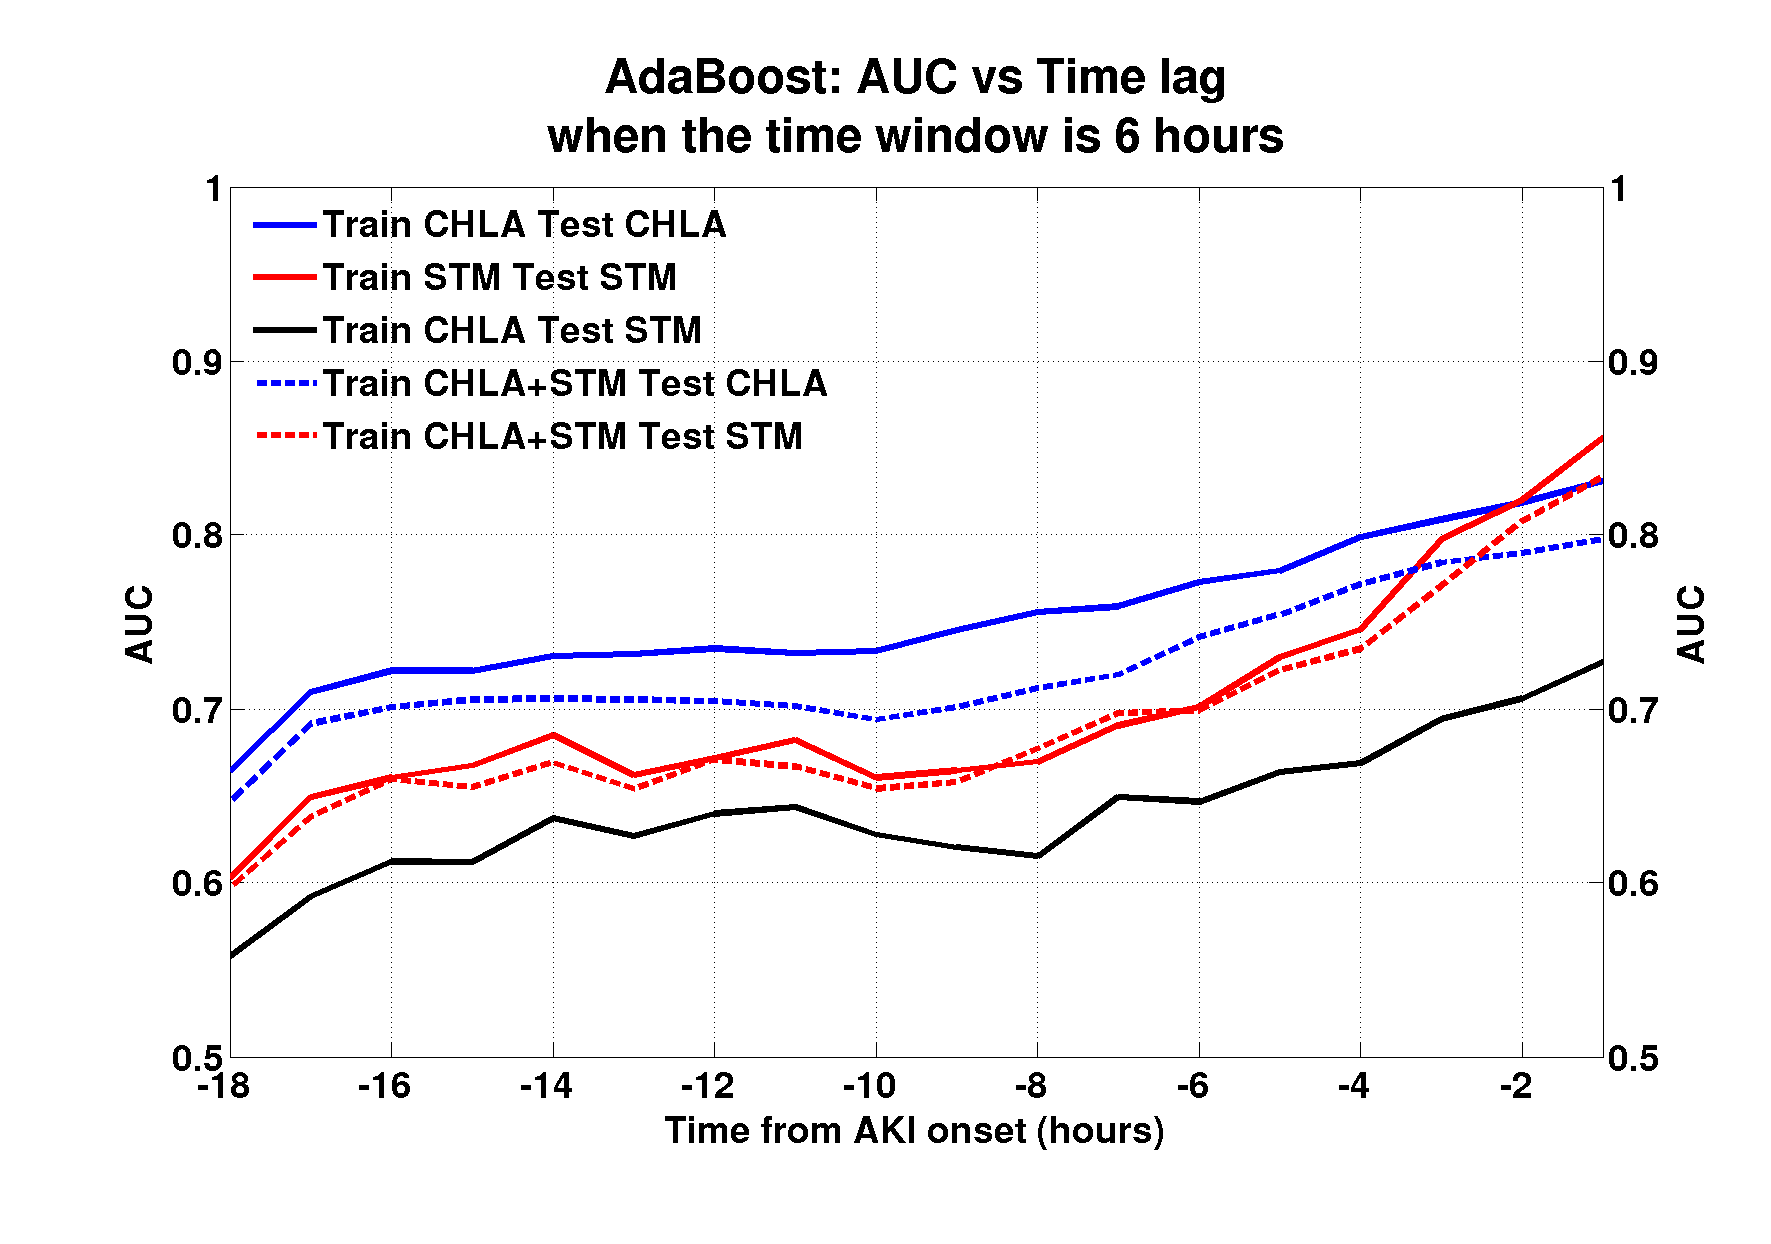
\includegraphics[width=\textwidth]{./figures/aucVStlag_twin006.png}
\caption{AUC comparison between models trained by data set from a single hospital or trained by a combined data set from two hospitals.} 
\label{fig:aucVStlag}      
\end{figure}


\section{Age Group Performance}
\label{sec:age_group_performance} 
In this section, we analyze the performances of the AdaBoost-abstain algorithm trained by different data sets. \fig{}\ref{fig:age_ism_ism} shows the test AUC over CHLA data set as a function of prediction window and age group of the AdaBoost-abstain algorithm trained by CHLA data set. AUC was higher for smaller prediction window as expected and AUC droped for younger age groups. This is because nearly 35 \% of the CHLA patients were older than 9 years old, whereas only 18 \% of the CHLA patients were younger than 6 months. Therefore, the algorithm tended to learn more by the older age groups. Similar trend was observed when the algorithm was trained by CHLA data set and tested on St.Mary's hospital data set. As shown in \fig{} \ref{fig:age_ism_stm}, approximately 10 \% AUC drop was observed over all age groups compard to the case when the algorithm was trained and tested on CHLA data set. This was consistent with the AUC drop observed in \fig{} \ref{fig:aucVStlag}. Except for the overall AUC drop, the algorithm showed similar prediction window size and age group dependency. The algorithm performed better for older age groups and short prediction window.

Next, we analyzed the age group performance for the algorithm trained by a combined data set from CHLA and St.Mary's hospital. Comparing \fig{} \ref{fig:age_across_ism}  and \fig{} \ref{fig:age_across_stm}, AUC drop was less than that when the algorithm was trained exclusiely by CHLA data set. This was consistent with the result shown in \fig{} \ref{fig:aucVStlag}. Another point to notice is that the algorithm generalized better over age groups when trained by a combined data set from CHLA and St.Mary's hospital. This is because approximately 22 \% of the patients in St.Mary's hospital were younger than 6 months, wheras only 17 \% of the patients were older than 9 years old. Since St.Mary's hospital had more patients in the younger group, the algorithm trained by combined data sets from CHLA and St.Mary's hospital generalized better over younger age groups.

\begin{figure}[!htbp]
\centering
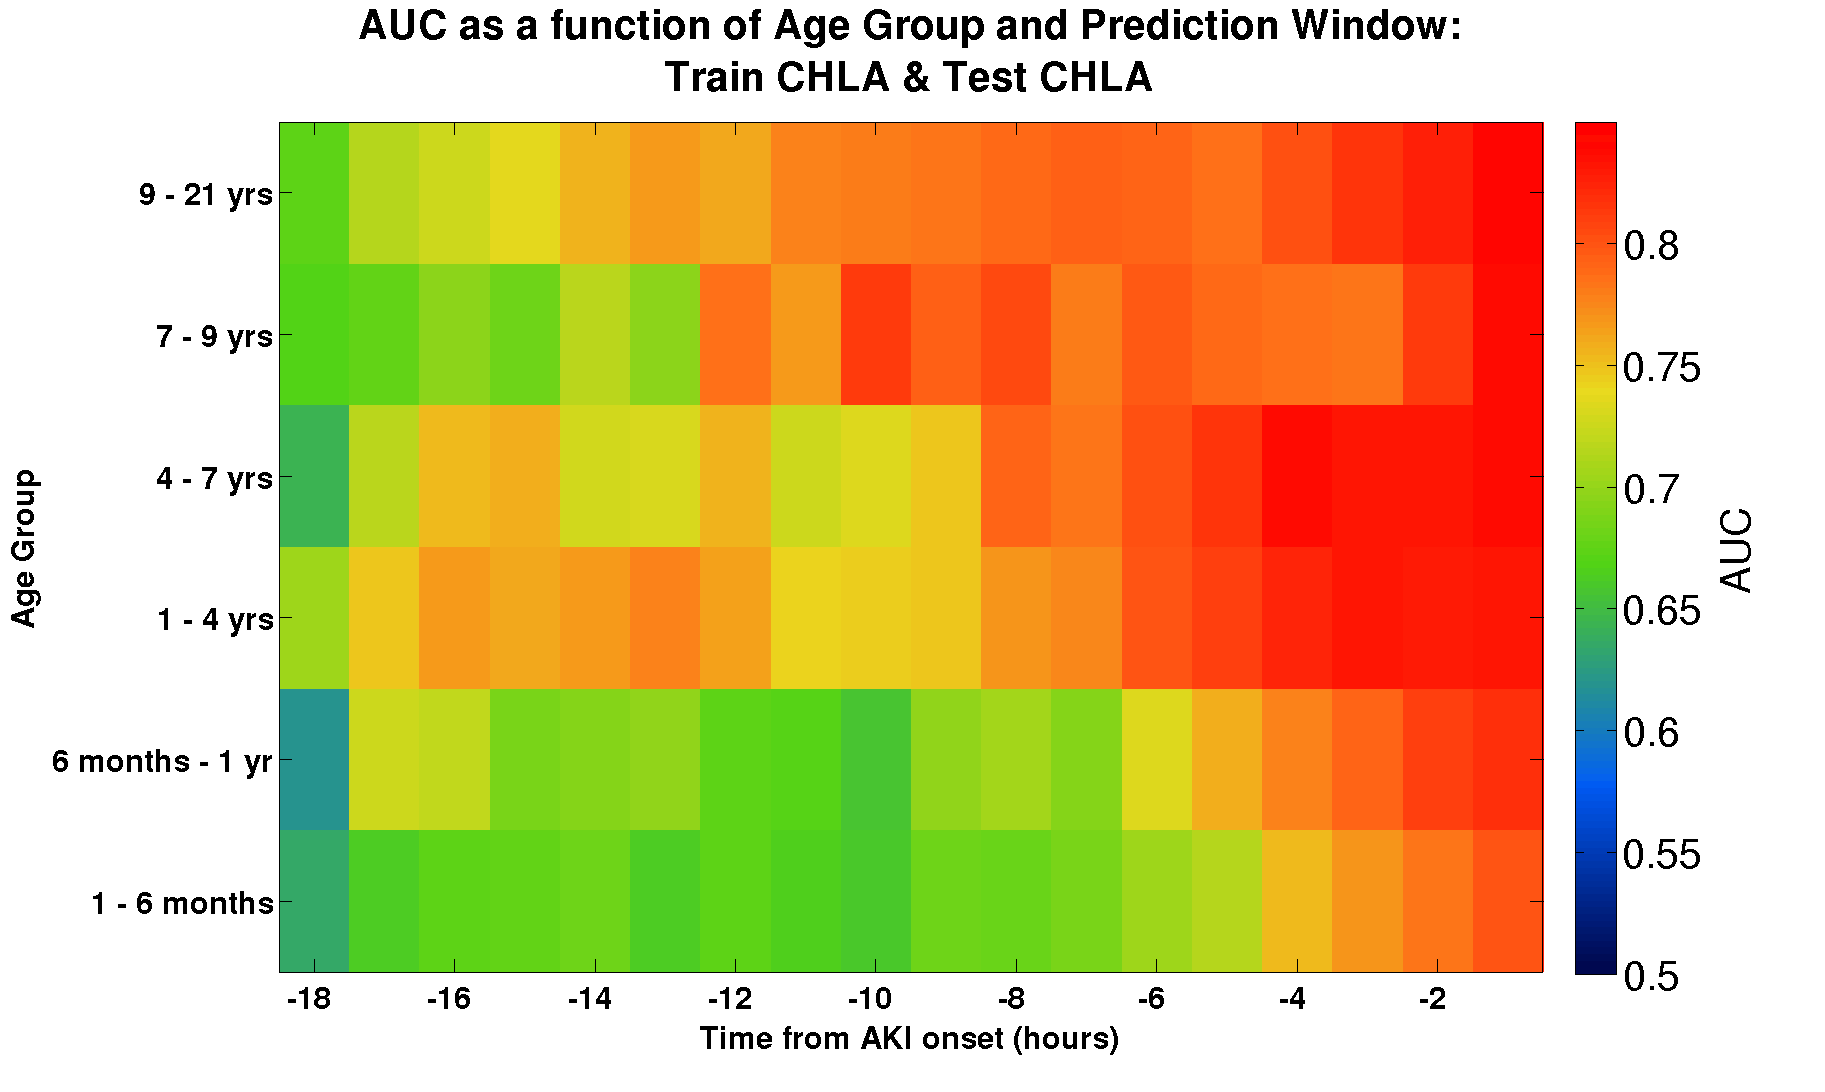
\includegraphics[width=\textwidth]{./figures/auc_age_ism_ism.png}
\caption{Test AUC over CHLA data set as a function of prediction window and age group of algorithm trained by CHLA data set} 
\label{fig:age_ism_ism}      
\end{figure}

\begin{figure}[!htbp]
\centering
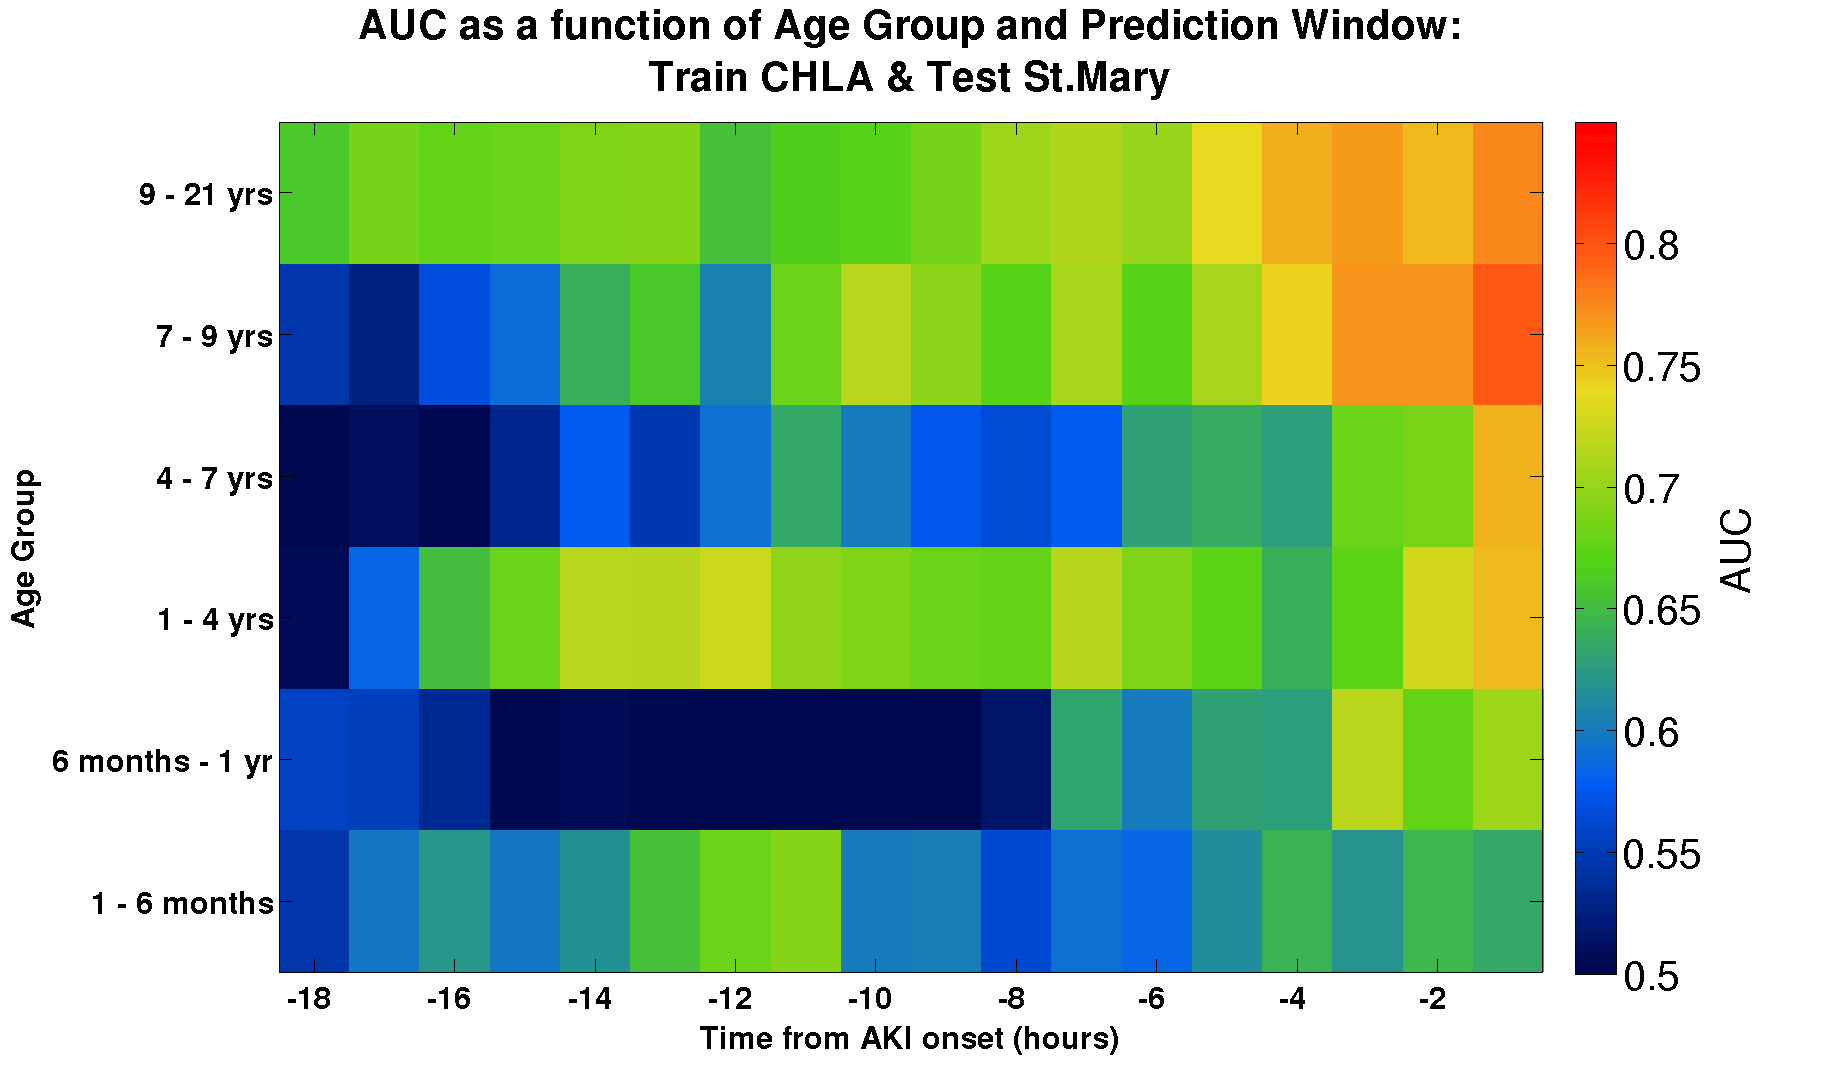
\includegraphics[width=\textwidth]{./figures/auc_age_ism_stm.png}
\caption{Test AUC over St.Mary's hospital data set as a function of prediction window and age group of algorithm trained by CHLA data set} 
\label{fig:age_ism_stm}      
\end{figure}

\begin{figure}[!htbp]
\centering
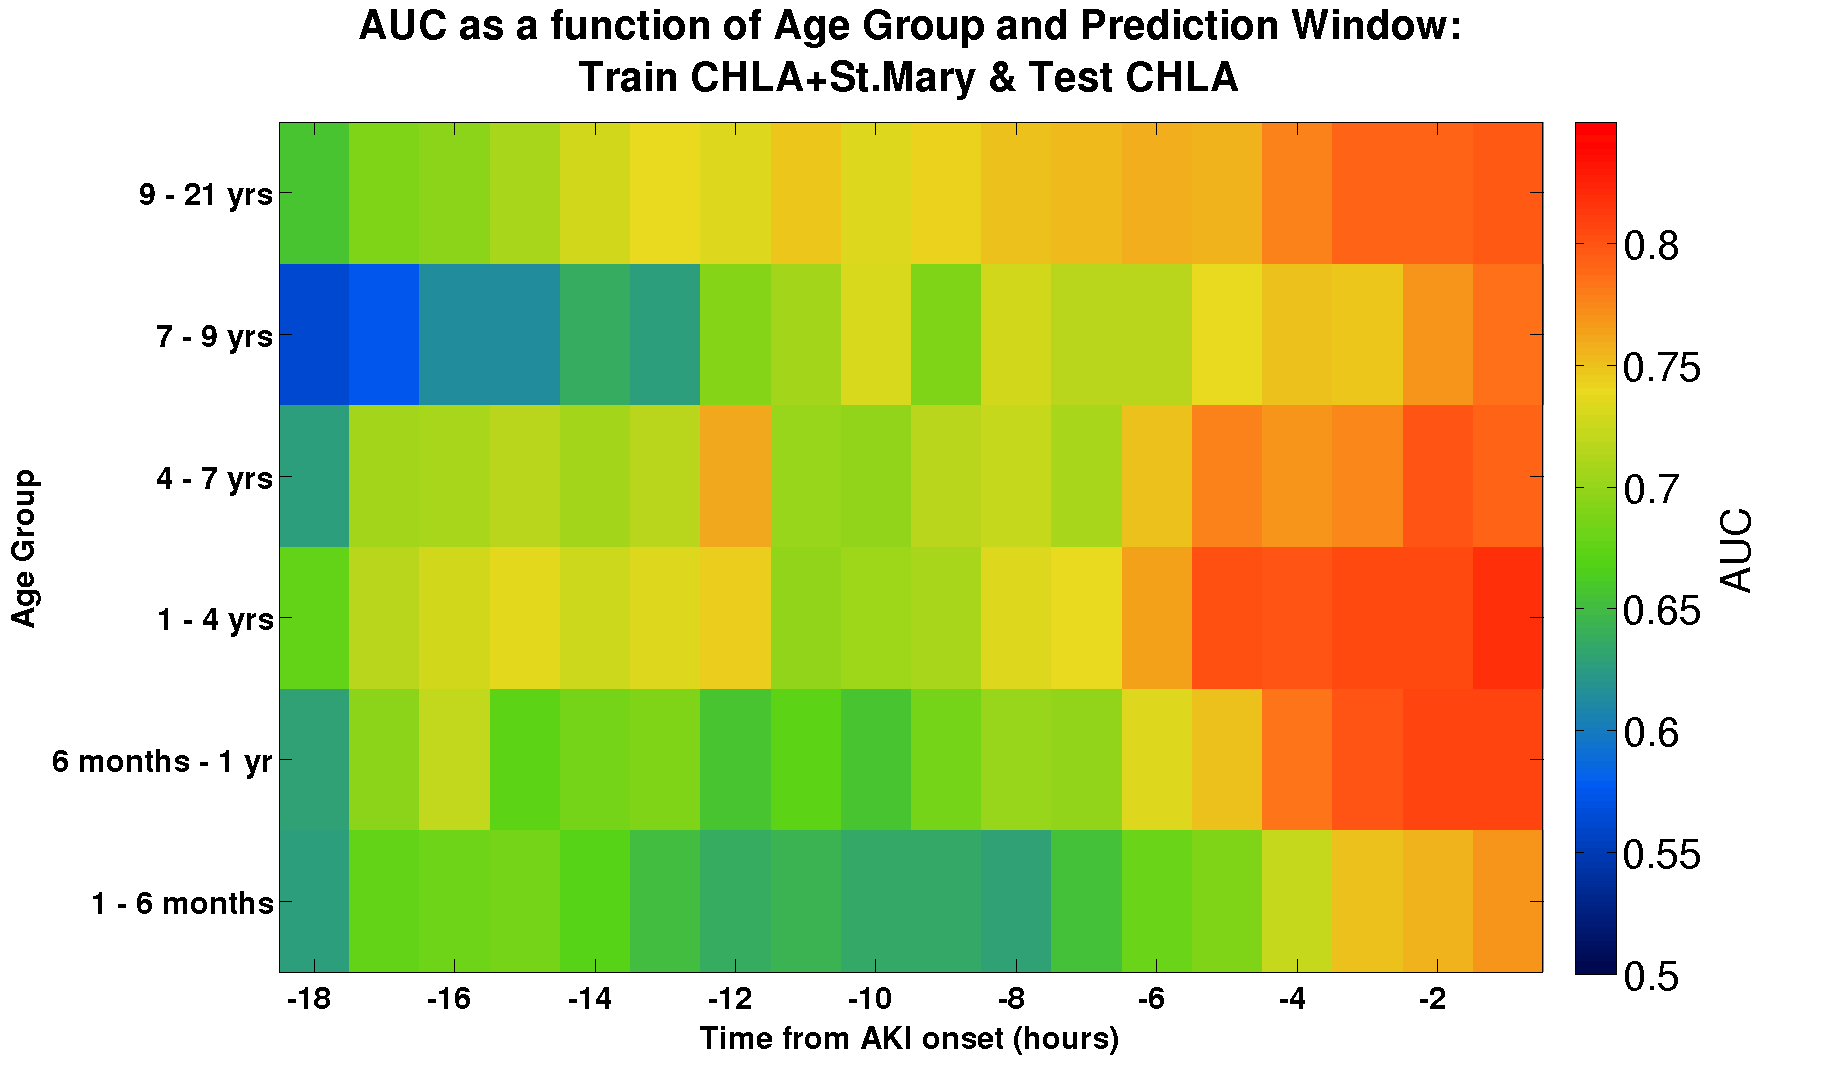
\includegraphics[width=\textwidth]{./figures/auc_age_across_ism.png}
\caption{Test AUC over CHLA data set as a function of prediction window and age group of algorithm trained by combined data set from CHLA and St.Mary's hospital} 
\label{fig:age_across_ism}      
\end{figure}

\begin{figure}[!htbp]
\centering
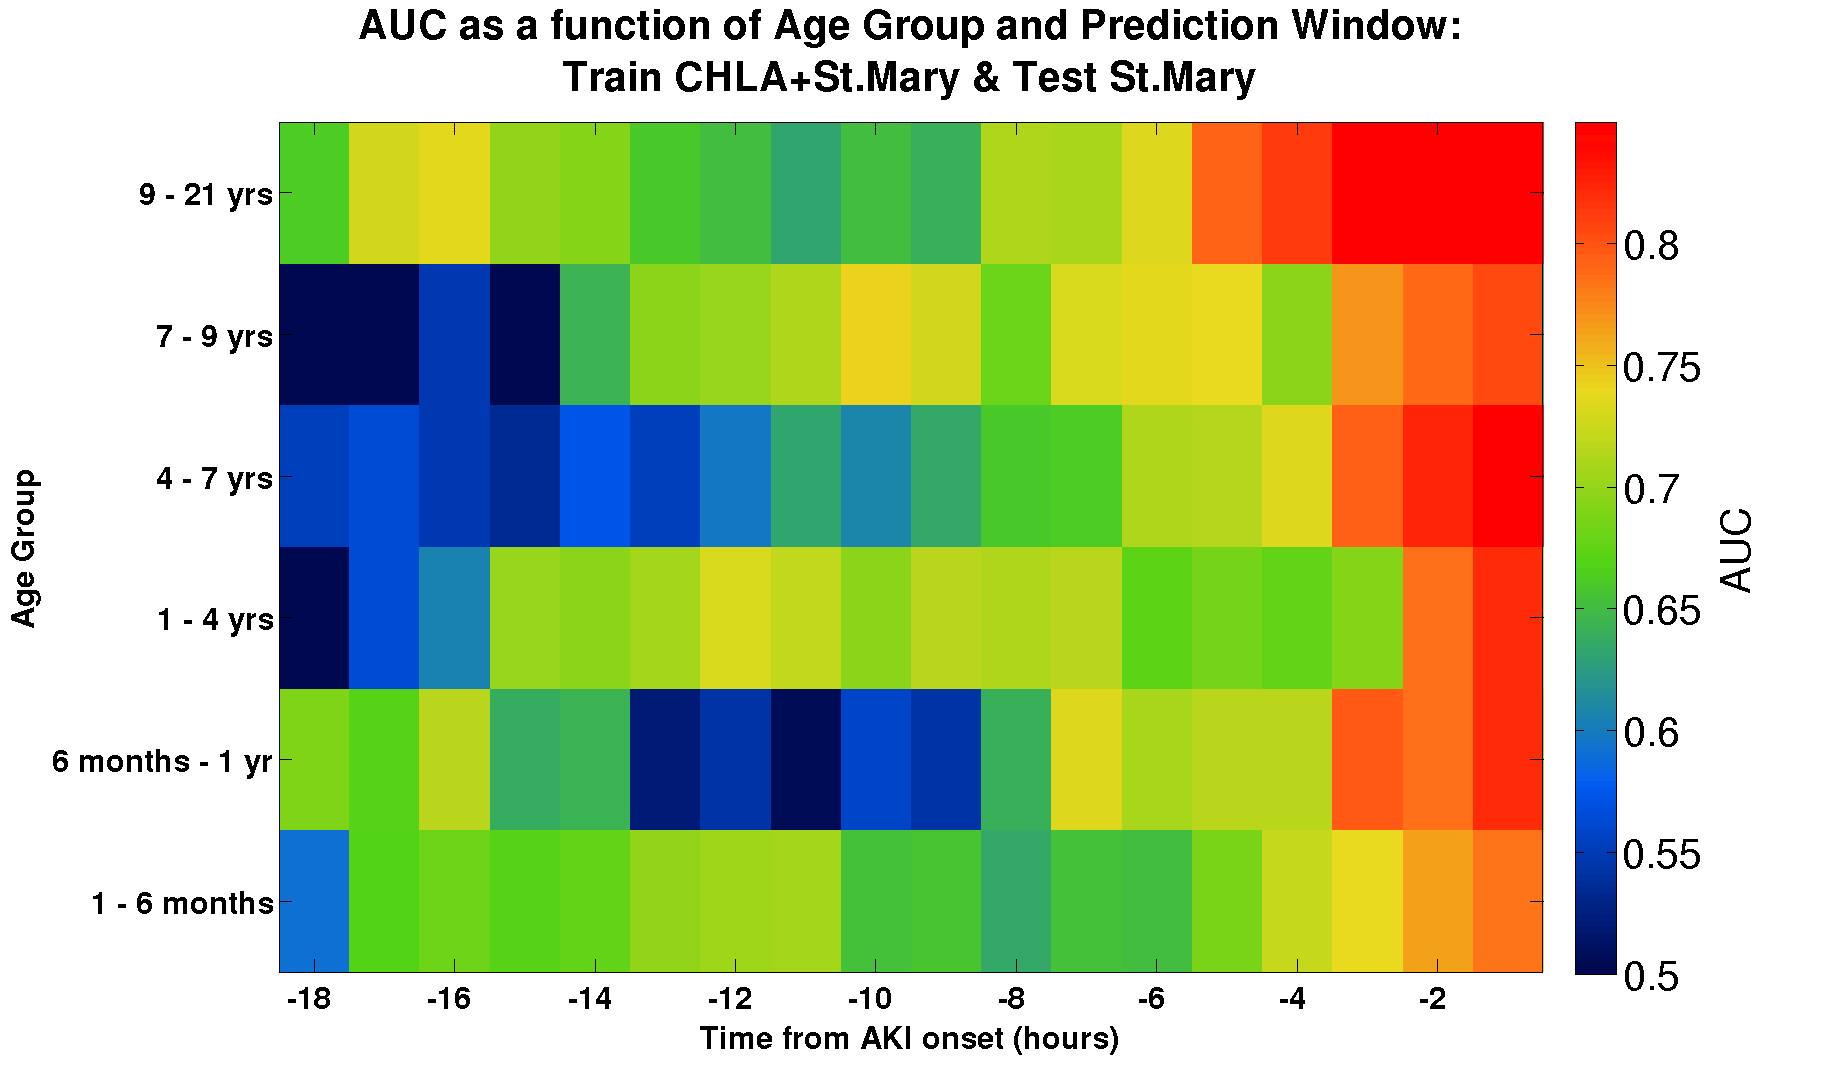
\includegraphics[width=\textwidth]{./figures/auc_age_across_stm.png}
\caption{Test AUC over St.Mary's hospital data set as a function of prediction window and age group of algorithm trained by combined data set from CHLA and St.Mary's hospital} 
\label{fig:age_across_stm}      
\end{figure}

\chapter{Discussion and Conclusion}
In this document, a binary classifier algorithm for early detection of AKI in pediatric ICU was described. Performance of the algorithm was analyzed for varying prediction window size. The algorithm was cross validated over different hospitals and showed better generalization performance among different hospitals and age groups when the algorithm was trained over a combined data set from different hospitals. The algorithm only takes most recent value of 18 features including vital signs, lab values, and demographics of the patient. This is highly advantageous for deployment because it requires only a small memory and CPU.

Since the algorithm was cross validated only over 3 hospitals, the algorithm should be cross validated over more hospitals and the performance should be checked in order to be more robust. Another research area is to find the baseline creatinine value for AKI staging. Though the AKI staging criteria is clearly defined, the criteria highly depends on patient's individual baseline creatinine. For the current implementation, a normal creatinine value for age and gender group is used as the baseline creatinine. However, the baseline creatinine value may vary among individual patients. Effectiveness of the algorithm should also be examined. For example, once the clinicians have information whether the patient may or may not develop AKI, we should examine what kind of treatments can be applied to prevent AKI, and how effective the treatments are.



\bibliography{pedAKIref}


\end{document}
